\documentclass[11pt]{article}

\usepackage[margin=1in]{geometry}
\usepackage{graphicx}
\usepackage{subcaption}
\usepackage{booktabs}
\usepackage{longtable}
\usepackage{array}
\usepackage{amsmath,amssymb}
\usepackage[hidelinks]{hyperref}
\usepackage{float}
\usepackage[section]{placeins}
\usepackage[dvipsnames]{xcolor}
\usepackage{tikz}
\usetikzlibrary{positioning, arrows.meta, fit, backgrounds, calc, shapes.geometric, decorations.pathreplacing}

\graphicspath{{figures/}{../}}

\newcommand{\UCILogo}{%
  \IfFileExists{uci_logo.png}{%
    
\includegraphics[width=0.62\linewidth]{uci_logo.png}%
  }{%
    \fbox{\parbox{0.3\linewidth}{\centering Missing UCI logo image}}%
  }%
}

\title{Stress Detection from Wearable Physiological Signals:\\A Multi-Model Analysis of the WESAD Dataset}
\author{Anishwar Chakraborty\\
\textit{Master of Data Science}\\
DATA 210P Statistical Methods}
\date{}

\begin{document}
\maketitle
\begin{center}
\vspace{-0.6em}
\UCILogo
\end{center}
\vspace{0.8em}

\tableofcontents
\newpage

% ======================================================================
\begin{abstract}
% ======================================================================
Chronic stress is a leading contributor to cardiovascular disease, anxiety disorders, and reduced quality of life, yet its detection remains largely reliant on subjective self-report.
Wearable physiological sensors offer an objective, continuous alternative, but translating raw signals into reliable stress predictions requires careful feature engineering, model selection, and subject-independent evaluation.

This project investigates automated stress detection using the WESAD (Wearable Stress and Affect Detection) dataset, a benchmark collection of multimodal physiological recordings from 15 subjects wearing wrist and chest sensors during controlled baseline, stress, and amusement protocols.
We pursue two complementary modelling strategies: (i)~tabular classification on hand-crafted window features using Logistic Regression, Random Forest, XGBoost, and a feed-forward MLP, and (ii)~deep sequence classification on raw time-series using standalone RNNs, standalone ResNets, and hybrid CNN-LSTM architectures with self-attention.
All models are evaluated under Leave-One-Subject-Out (LOSO) cross-validation to ensure metrics reflect genuine cross-subject generalisation.

On engineered features, the MLP achieves the best binary stress detection (Macro-F1 = 0.898), while XGBoost leads 3-class classification (Macro-F1 = 0.677).
Standalone RNNs and ResNets on raw 30-second windows yield 0.60--0.79 accuracy, indicating that naive end-to-end learning on low-rate wrist signals is insufficient.
Our improved pipeline---60-second overlapping windows, per-subject normalisation, and hybrid CNN-LSTM with self-attention---raises raw-signal accuracy meaningfully, demonstrating that combining local convolutional feature extraction with temporal recurrent modelling and attention-based pooling bridges much of the gap between hand-crafted and learned representations.
\end{abstract}

% ======================================================================
\section{Introduction}
\label{sec:intro}
% ======================================================================

Psychological stress activates the hypothalamic-pituitary-adrenal (HPA) axis and the autonomic nervous system, producing measurable changes in skin conductance, heart rate, peripheral temperature, respiration, and motor activity~\cite{schmidt2018wesad}.
With the proliferation of wrist-worn wearable devices capable of recording these signals continuously, automated stress detection has become a feasible goal with applications in occupational health, mental wellness monitoring, and clinical decision support~\cite{can2019stress}.

\subsection{Aims and Goals}

The aims of this project are threefold:
\begin{enumerate}    \item \textbf{Explore and characterise} the WESAD dataset through rigorous exploratory data analysis, identifying class imbalance, inter-subject variability, feature separability, and potential confounds.
    \item \textbf{Develop and compare} multiple classification pipelines---from interpretable linear baselines through gradient-boosted trees and neural networks on engineered features, to deep sequence models on raw wrist signals---using subject-independent LOSO evaluation.
    \item \textbf{Investigate improved deep learning architectures} (CNN-LSTM hybrids with attention and multi-scale convolutions) to determine whether end-to-end learning from raw wrist signals can match or exceed hand-crafted feature pipelines.
\end{enumerate}


% ======================================================================
\section{Literature Review}
\label{sec:litreview}
% ======================================================================

\subsection{The WESAD Benchmark}
Schmidt et al.~\cite{schmidt2018wesad} introduced WESAD as a publicly available multimodal dataset for wearable stress and affect detection, recording 15 subjects with both a chest-worn RespiBAN (ECG, EDA, EMG, respiration, temperature, acceleration at 700\,Hz) and a wrist-worn Empatica E4 (BVP at 64\,Hz, EDA at 4\,Hz, temperature at 4\,Hz, acceleration at 32\,Hz).
Using AdaBoost and Linear Discriminant Analysis on hand-crafted features, they reported up to 80\% accuracy for 3-class and 93\% for binary (stress vs.\ non-stress) classification.

\subsection{Traditional Machine Learning for Stress Detection}
Subsequent work explored a range of classical models on WESAD.
Siirtola~\cite{siirtola2019continuous} applied Random Forest with reduced HRV feature sets and achieved strong results under person-specific evaluation, though cross-subject performance was notably lower.
Bobade and Vani~\cite{bobade2020stress} compared Decision Trees, Random Forests, and XGBoost on wearable features, finding that gradient-boosted ensembles consistently outperformed bagging methods on physiological data, particularly for minority-class detection.
A systematic review by Can et al.~\cite{can2019stress} noted that electrodermal activity and heart rate variability are the most discriminative modalities, and that Leave-One-Subject-Out (LOSO) cross-validation is essential for estimating real-world generalisation.

\subsection{Deep Learning on Raw Physiological Signals}
More recently, deep learning approaches have been applied directly to raw time-series.
Sano et al.~\cite{sano2023cnnlstm} demonstrated that hybrid CNN-LSTM architectures outperform standalone RNNs for stress detection from PPG signals, achieving approximately 97\% accuracy on the WESAD dataset using 5-second PPG segments.
Lin et al.~\cite{lin2023selfattention} showed that self-attention mechanisms applied to LSTM outputs improve classification of physiological time-series by learning to weight informative time steps, with a CNN-BiLSTM-Attention model achieving 99.46\% on EEG state classification.
For 1D time-series, Fawaz et al.~\cite{fawaz2019resnet} demonstrated that residual networks achieve state-of-the-art results on the UCR time-series benchmark, often matching or exceeding RNN-based methods while training faster due to the absence of sequential dependencies.

\subsection{Gaps Addressed by This Work}
Despite these advances, most WESAD studies either (a)~use chest sensors (unavailable in consumer wearables), (b)~evaluate with random splits rather than LOSO, or (c)~test only one modelling paradigm.
This project addresses all three gaps: we use only wrist-sensor data, enforce strict LOSO evaluation throughout, and systematically compare tabular, RNN, ResNet, and hybrid CNN-LSTM approaches within a single framework.


% ======================================================================
\section{Data Introduction}
\label{sec:data}
% ======================================================================

\subsection{Dataset Overview}
The WESAD dataset comprises recordings from 15 subjects (S2--S17, excluding S1 and S12) who underwent a laboratory protocol consisting of baseline (seated rest), stress (Trier Social Stress Test), and amusement (watching funny video clips) conditions.
Each subject's session lasts approximately 2 hours, producing continuous multi-sensor recordings with synchronised condition labels sampled at 700\,Hz.

\subsection{Sensor Modalities and Derived Features}
We use only the \textbf{wrist-worn Empatica E4} signals:
\begin{itemize}
    \item \textbf{EDA (Electrodermal Activity)} (4\,Hz): skin conductance reflecting sympathetic nervous system activity. EDA is further decomposed into:
    \begin{itemize}
        \item \textbf{Phasic component}: fast skin conductance responses (SCRs), directly linked to arousal events.
        \item \textbf{Tonic component}: slow baseline level (SCL), capturing longer-term drift.
        \item \textbf{SMNA / sparse driver}: estimated event-like driver activity from the decomposition.
    \end{itemize}
    \item \textbf{BVP (Blood Volume Pulse)} (64\,Hz): optical photoplethysmography signal carrying heart-beat periodicity but highly sensitive to motion artifacts and poor sensor contact.
    \item \textbf{BVP peak frequency}: dominant frequency in the BVP window (from a periodogram), a proxy for heart-rate band behaviour.
    \item \textbf{TEMP (Skin Temperature)} (4\,Hz): usually changes slowly; more informative through trends (slope) than rapid fluctuations.
    \item \textbf{ACC (Accelerometer)} (32\,Hz): 3-axis wrist acceleration measuring movement intensity and posture changes. Important both as a predictor and as an artifact indicator.
    \item \textbf{net\_acc}: acceleration magnitude ($\approx\sqrt{x^2+y^2+z^2}$) summarised over a window; a compact motion intensity feature.
    \item \textbf{Resp (Respiration)}: breathing signal from the chest device; stress can change breathing rate and variability.
\end{itemize}

\subsection{Data Transformation Pipeline}
Raw WESAD recordings are multi-rate time series. The transformation pipeline converts them into a window-level feature table:
\begin{enumerate}
    \item \textbf{Load raw wrist/chest signals and labels.}
    \item \textbf{Denoise signals} via smoothing / low-pass filtering to reduce high-frequency noise.
    \item \textbf{Time-align modalities.} Signals sampled at different rates are aligned onto a consistent timeline; labels are propagated so every aligned time point has an associated class.
    \item \textbf{EDA decomposition (cvxEDA).} EDA is decomposed into tonic (slow drift) and phasic (fast SCR-like responses) components.
    \item \textbf{Split into protocol segments} (baseline / stress / amusement) using the synchronised label stream.
    \item \textbf{Windowing.} The continuous signal is partitioned into \textbf{30-second} fixed windows, creating labelled examples.
    \item \textbf{Feature extraction per window.} For each sensor channel, compute summary statistics (mean, std, min, max) plus domain-engineered features (BVP dominant frequency, temperature slope, ACC magnitude).
\end{enumerate}

% --- DATA PIPELINE FIGURE ---
\begin{figure}[H]
\centering
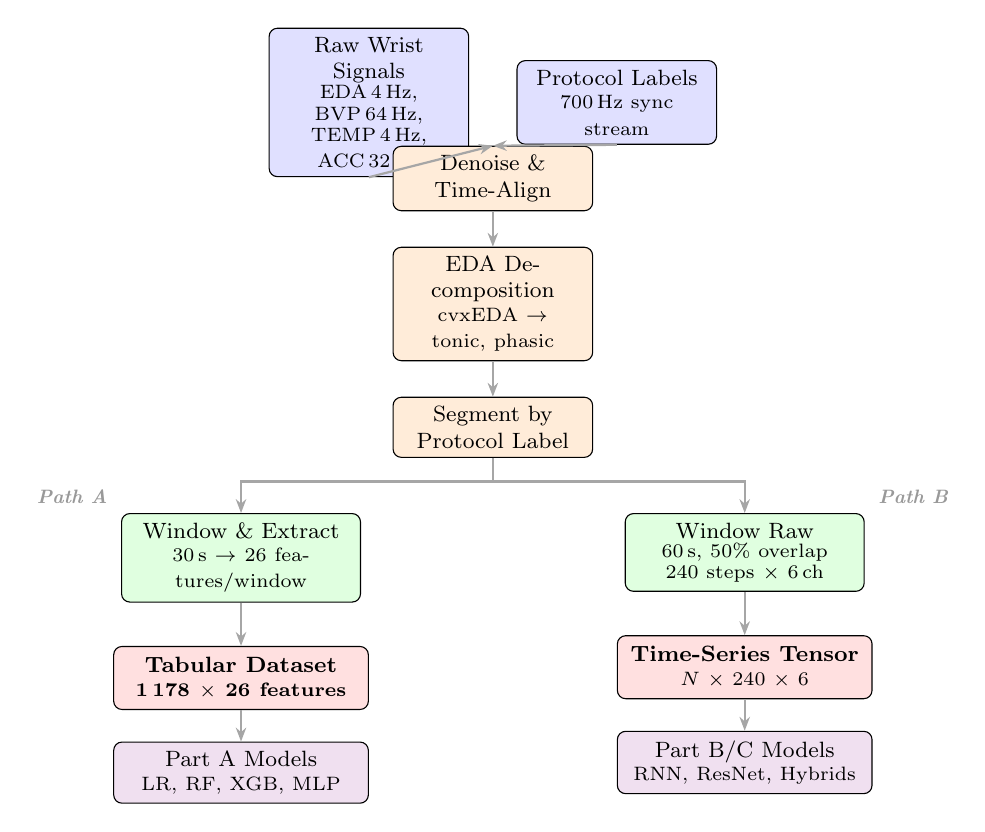
\begin{tikzpicture}[
    node distance=0.45cm and 0.6cm,
    box/.style={draw, rounded corners=3pt, minimum height=0.7cm,
                text width=2.3cm, align=center, font=\footnotesize},
    raw/.style={box, fill=blue!12},
    proc/.style={box, fill=orange!15},
    split/.style={box, fill=green!12, text width=2.8cm},
    outbox/.style={box, fill=red!12, text width=3.0cm, minimum height=0.8cm, font=\footnotesize\bfseries},
    arr/.style={-{Stealth[length=5pt]}, thick, color=gray!70},
    pathlbl/.style={font=\scriptsize\itshape, text=gray!80},
]
% Row 1: raw inputs
\node[raw] (rawin) {Raw Wrist Signals\\[-1pt]\scriptsize EDA\,4\,Hz, BVP\,64\,Hz,\\[-2pt]\scriptsize TEMP\,4\,Hz, ACC\,32\,Hz};
\node[raw, right=of rawin] (labels) {Protocol Labels\\[-1pt]\scriptsize 700\,Hz sync stream};

% Row 2: preprocessing
\node[proc, below=0.55cm of $(rawin)!0.5!(labels)$] (denoise) {Denoise \&\\Time-Align};
\draw[arr] (rawin.south) -- (denoise.north);
\draw[arr] (labels.south) -- (denoise.north);

\node[proc, below=of denoise] (eda) {EDA Decomposition\\[-1pt]\scriptsize cvxEDA $\to$ tonic, phasic};
\draw[arr] (denoise) -- (eda);

\node[proc, below=of eda] (segment) {Segment by\\Protocol Label};
\draw[arr] (eda) -- (segment);

% Split into two paths
\node[split, below left=0.7cm and 0.4cm of segment] (win30) {Window \& Extract\\[-1pt]\scriptsize 30\,s $\to$ 26 features/window};
\node[split, below right=0.7cm and 0.4cm of segment] (win60) {Window Raw\\[-1pt]\scriptsize 60\,s, 50\% overlap\\[-2pt]\scriptsize 240 steps $\times$ 6\,ch};

\draw[arr] (segment.south) -- ++(0,-0.3) -| (win30.north);
\draw[arr] (segment.south) -- ++(0,-0.3) -| (win60.north);

% Outputs
\node[outbox, below=0.55cm of win30] (tabular) {Tabular Dataset\\[-1pt]\scriptsize 1\,178 $\times$ 26 features};
\node[outbox, below=0.55cm of win60] (tensor) {Time-Series Tensor\\[-1pt]\scriptsize $N \times 240 \times 6$};
\draw[arr] (win30) -- (tabular);
\draw[arr] (win60) -- (tensor);

% Model destinations
\node[box, fill=violet!12, below=0.4cm of tabular, text width=3.0cm] (mA) {Part A Models\\[-1pt]\scriptsize LR, RF, XGB, MLP};
\node[box, fill=violet!12, below=0.4cm of tensor, text width=3.0cm] (mBC) {Part B/C Models\\[-1pt]\scriptsize RNN, ResNet, Hybrids};
\draw[arr] (tabular) -- (mA);
\draw[arr] (tensor) -- (mBC);

% path labels
\node[pathlbl, left=0.05cm of win30.north west, anchor=south east] {\textbf{Path A}};
\node[pathlbl, right=0.05cm of win60.north east, anchor=south west] {\textbf{Path B}};

\end{tikzpicture}
\caption{End-to-end data processing pipeline. Raw multi-rate wrist signals are denoised, time-aligned, and decomposed, then split into two parallel paths: \textbf{Path A} extracts hand-crafted summary features for tabular classifiers (Part~A), while \textbf{Path B} produces raw time-series tensors for deep sequence models (Parts~B and C).}
\label{fig:pipeline}
\end{figure}

\subsubsection{Why Summary Statistics are Used as Features}
Window features compress high-frequency signals into stable vectors that capture the window's overall level, variability, and extremes:
\begin{itemize}
    \item \textbf{Mean}: arithmetic average; captures typical signal level but is sensitive to spikes/outliers.
    \item \textbf{Standard deviation}: within-window variability (often rises with motion artifacts in BVP).
    \item \textbf{Min/max}: extremes reflecting physiological peaks or sensor artifacts.
    \item \textbf{Slope}: monotonic trends (e.g., temperature drifting).
    \item \textbf{Peak frequency}: dominant periodic structure (useful for BVP).
\end{itemize}

\subsection{Metadata Parsing and Merging}
Subjects differ in demographic and contextual factors (age, gender, smoking, etc.). These fields are extracted from per-subject metadata and encoded as model-ready columns (e.g., one-hot indicators) to support interpretation and confound analysis.

\subsection{Engineered Feature Dataset}
Each row corresponds to one \textbf{30-second window} from one subject, represented by engineered window features plus a class label and metadata.
The resulting dataset contains \textbf{1{,}178 windows} across 15 subjects.
Two feature sets are defined: \textbf{sensor-only} (26 features) and \textbf{sensor+demographics} (29 features).

\subsubsection{Label Meanings}
\begin{center}
\begin{tabular}{cl}
\toprule
\textbf{Label value} & \textbf{Meaning} \\
\midrule
0 & Amusement (195 windows, 16.6\%) \\
1 & Baseline (628 windows, 53.3\%) \\
2 & Stress (355 windows, 30.1\%) \\
\bottomrule
\end{tabular}
\end{center}

\subsubsection{Sample Rows}

\begin{table}[H]
  \centering
  \small
  \begin{tabular}{@{}rrrrrrrrr@{}}
    \toprule
    idx & subject & label & EDA\_mean & EDA\_phasic\_mean & BVP\_std & TEMP\_mean & Resp\_std & net\_acc\_mean \\
    \midrule
    0 & 2 & 1 & 1.398 & 1.829 & 107.679 & 35.817 & 0.011 & 0.026 \\
    1 & 2 & 1 & 1.210 & 2.111 & 118.776 & 35.798 & 0.021 & 0.029 \\
    2 & 2 & 1 & 1.011 & 0.153 & 42.202 & 35.713 & 0.011 & 0.033 \\
    3 & 2 & 1 & 0.775 & 0.178 & 41.619 & 35.701 & 0.003 & 0.018 \\
    \bottomrule
  \end{tabular}
  \caption{Sample windows from the engineered feature dataset (representative subset of columns).}
  \label{tab:samples}
\end{table}

\subsubsection{Column-by-Column Explanation}

\renewcommand{\arraystretch}{1.1}
\begin{longtable}{@{}p{0.30\textwidth}p{0.65\textwidth}@{}}
\caption{\label{tab:columns}Column headers in the engineered feature dataset and their meaning.}\\
\toprule
\textbf{Column} & \textbf{Meaning} \\
\midrule
\endfirsthead
\toprule
\textbf{Column} & \textbf{Meaning} \\
\midrule
\endhead
\bottomrule
\endfoot

\texttt{EDA\_mean} & Mean of wrist electrodermal activity (EDA) in the window. \\
\texttt{EDA\_std} & Standard deviation of EDA in the window. \\
\texttt{EDA\_min} & Minimum EDA in the window. \\
\texttt{EDA\_max} & Maximum EDA in the window. \\

\texttt{EDA\_phasic\_mean} & Mean of the phasic EDA component (fast responses) in the window. \\
\texttt{EDA\_phasic\_std} & Std of the phasic EDA component in the window. \\
\texttt{EDA\_phasic\_min} & Minimum of the phasic EDA component in the window. \\
\texttt{EDA\_phasic\_max} & Maximum of the phasic EDA component in the window. \\

\texttt{EDA\_smna\_mean} & Mean of the sparse driver component from EDA decomposition. \\
\texttt{EDA\_smna\_std} & Std of the sparse driver component in the window. \\
\texttt{EDA\_smna\_min} & Minimum of the sparse driver component in the window. \\
\texttt{EDA\_smna\_max} & Maximum of the sparse driver component in the window. \\

\texttt{EDA\_tonic\_mean} & Mean of the tonic EDA component (slow drift / baseline level). \\
\texttt{EDA\_tonic\_std} & Std of the tonic EDA component in the window. \\
\texttt{EDA\_tonic\_min} & Minimum of the tonic EDA component in the window. \\
\texttt{EDA\_tonic\_max} & Maximum of the tonic EDA component in the window. \\

\texttt{BVP\_mean} & Mean of wrist blood volume pulse (BVP) in the window. \\
\texttt{BVP\_std} & Std of BVP in the window (often increases with motion artifacts). \\
\texttt{BVP\_min} & Minimum BVP in the window. \\
\texttt{BVP\_max} & Maximum BVP in the window. \\

\texttt{TEMP\_mean} & Mean wrist skin temperature in the window. \\
\texttt{TEMP\_std} & Std of temperature in the window. \\
\texttt{TEMP\_min} & Minimum temperature in the window. \\
\texttt{TEMP\_max} & Maximum temperature in the window. \\

\texttt{ACC\_x/y/z\_mean} & Mean wrist acceleration per axis in the window. \\
\texttt{ACC\_x/y/z\_std} & Std wrist acceleration per axis in the window. \\
\texttt{ACC\_x/y/z\_min} & Minimum wrist acceleration per axis in the window. \\
\texttt{ACC\_x/y/z\_max} & Maximum wrist acceleration per axis in the window. \\

\texttt{Resp\_mean} & Mean respiration signal in the window. \\
\texttt{Resp\_std} & Std respiration signal in the window. \\
\texttt{Resp\_min} & Minimum respiration signal in the window. \\
\texttt{Resp\_max} & Maximum respiration signal in the window. \\

\texttt{net\_acc\_mean/std/min/max} & Acceleration magnitude summary statistics. \\
\texttt{BVP\_peak\_freq} & Dominant frequency of BVP in the window (periodogram peak). \\
\texttt{TEMP\_slope} & Linear temperature trend across the window. \\

\texttt{subject} & Subject identifier (integer). \\
\texttt{label} & Window label (0=amusement, 1=baseline, 2=stress). \\

\texttt{age} & Subject age. \\
\texttt{height} & Subject height. \\
\texttt{weight} & Subject weight. \\

\texttt{gender\_female/male} & One-hot gender indicators. \\
\texttt{coffee\_today\_YES} & One-hot: drank coffee today. \\
\texttt{sport\_today\_YES} & One-hot: did sports today. \\
\texttt{smoker\_NO/YES} & One-hot: smoking status. \\
\texttt{feel\_ill\_today\_YES} & One-hot: feels ill today. \\

\end{longtable}

\subsection{Raw Time-Series Data}
For deep sequence models, raw wrist signals are loaded from per-subject data files, resampled to a common 4\,Hz, and segmented into fixed-length windows.
Two windowing strategies are evaluated:
\begin{itemize}
    \item \textbf{Baseline}: 30-second non-overlapping windows (120 time steps $\times$ 6 channels), yielding $\sim$1{,}178 windows.
    \item \textbf{Improved}: 60-second windows with 50\% overlap (240 time steps $\times$ 6 channels), yielding $\sim$1{,}105 windows with richer temporal context.
\end{itemize}

% --- WINDOWING COMPARISON FIGURE ---
\begin{figure}[H]
\centering
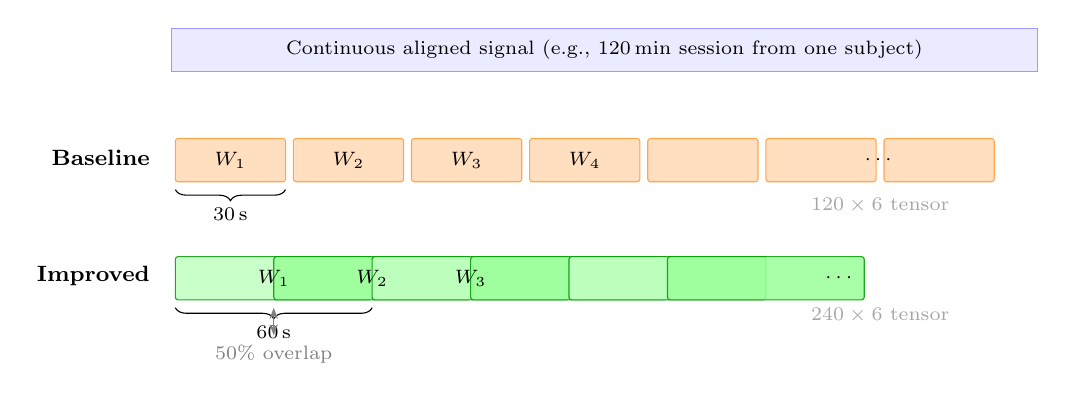
\begin{tikzpicture}[
    font=\footnotesize,
    signal/.style={fill=blue!8, draw=blue!40, minimum height=0.55cm},
    winA/.style={fill=orange!25, draw=orange!70, minimum height=0.55cm, rounded corners=1pt},
    winB/.style={fill=green!20, draw=green!60!black, minimum height=0.55cm, rounded corners=1pt},
    brace/.style={decorate, decoration={brace, amplitude=4pt, mirror}},
    lbl/.style={font=\scriptsize, text=gray!70},
]
% Continuous signal bar
\fill[blue!8, draw=blue!40] (0,0) rectangle (11,0.55);
\node[font=\scriptsize] at (5.5,0.275) {Continuous aligned signal (e.g., 120\,min session from one subject)};

% --- Baseline: 30s non-overlapping ---
\node[anchor=east, font=\footnotesize\bfseries] at (-0.15,-1.1) {Baseline};
\foreach \i in {0,1,...,6} {
    \fill[orange!25, draw=orange!70, rounded corners=1pt]
        (\i*1.5+0.05, -1.4) rectangle (\i*1.5+1.45, -0.85);
}
\node[font=\scriptsize] at (0.75,-1.125) {$W_1$};
\node[font=\scriptsize] at (2.25,-1.125) {$W_2$};
\node[font=\scriptsize] at (3.75,-1.125) {$W_3$};
\node[font=\scriptsize] at (5.25,-1.125) {$W_4$};
\node[font=\scriptsize] at (9.0,-1.125) {$\cdots$};
\draw[brace] (0.05,-1.5) -- (1.45,-1.5) node[midway, below=3pt, font=\scriptsize] {30\,s};

% --- Improved: 60s with 50% overlap ---
\node[anchor=east, font=\footnotesize\bfseries] at (-0.15,-2.6) {Improved};
\foreach \i in {0,1,...,5} {
    \pgfmathsetmacro{\startx}{\i*1.25+0.05}
    \pgfmathsetmacro{\endx}{\i*1.25+2.55}
    \pgfmathsetmacro{\op}{25+mod(\i,2)*15}
    \fill[green!\op, draw=green!60!black, rounded corners=1pt, opacity=0.85]
        (\startx, -2.9) rectangle (\endx, -2.35);
}
\node[font=\scriptsize] at (1.3,-2.625) {$W_1$};
\node[font=\scriptsize] at (2.55,-2.625) {$W_2$};
\node[font=\scriptsize] at (3.80,-2.625) {$W_3$};
\node[font=\scriptsize] at (8.5,-2.625) {$\cdots$};
\draw[brace] (0.05,-3.0) -- (2.55,-3.0) node[midway, below=3pt, font=\scriptsize] {60\,s};
\draw[{Stealth[length=4pt]}-{Stealth[length=4pt]}, gray] (1.30,-3.0) -- (1.30,-3.35)
    node[below, font=\scriptsize, text=gray] {50\% overlap};

% annotations
\node[lbl, anchor=west] at (8.0, -1.7) {$120 \times 6$ tensor};
\node[lbl, anchor=west] at (8.0, -3.1) {$240 \times 6$ tensor};

\end{tikzpicture}
\caption{Windowing strategies for raw time-series input. \textbf{Baseline}: 30-second non-overlapping windows produce $120 \times 6$ tensors. \textbf{Improved}: 60-second windows with 50\% overlap produce $240 \times 6$ tensors, providing richer temporal context and more training examples through data augmentation.}
\label{fig:windowing}
\end{figure}


% ======================================================================
\section{Exploratory Data Analysis}
\label{sec:eda}
% ======================================================================

The EDA is designed to answer three modelling-critical questions:
\begin{enumerate}
  \item \textbf{Is the dataset balanced and comparable across subjects?}
  \item \textbf{Do features separate the classes, and which modalities matter most?}
  \item \textbf{Are there artifacts/outliers or subject-specific effects that will hurt generalisation?}
\end{enumerate}

% ------------------------------------------------------------------
\subsection{Dataset Composition and Balance}
% ------------------------------------------------------------------

\begin{figure}[H]
  \centering
  \begin{subfigure}{0.49\linewidth}
    \centering
    \includegraphics[width=\linewidth]{\detokenize{eda_outputs_m14/01_label_counts.png}}
    \caption{Overall class balance.}
  \end{subfigure}
  \hfill
  \begin{subfigure}{0.49\linewidth}
    \centering
    \includegraphics[width=\linewidth]{\detokenize{eda_outputs_m14/02_windows_per_subject_stacked.png}}
    \caption{Per-subject window counts split by label.}
  \end{subfigure}
  \caption{Composition plots used to assess imbalance and protocol consistency.}
  \label{fig:composition}
\end{figure}

The dataset is moderately imbalanced: Baseline (628 windows, 53.3\%) outnumbers Amusement (195 windows, 16.6\%) by 3.2:1.
The per-subject stacked bar chart confirms that every subject contributes all three classes in roughly consistent proportions, reflecting the standardised protocol.
However, the imbalance means that accuracy alone is misleading---a model that always predicts Baseline would achieve 53\% accuracy.
This motivates the use of \textbf{class-weighted loss functions} and \textbf{Macro-F1} as the primary evaluation metric.

% ------------------------------------------------------------------
\subsection{Univariate Feature Separation by Label}
% ------------------------------------------------------------------

\begin{figure}[H]
  \centering
  \begin{subfigure}{0.49\linewidth}
    \centering
    \includegraphics[width=\linewidth]{\detokenize{eda_outputs_m14/03_box_eda_mean_by_label.png}}
    \caption{EDA mean by label.}
  \end{subfigure}
  \hfill
  \begin{subfigure}{0.49\linewidth}
    \centering
    \includegraphics[width=\linewidth]{\detokenize{eda_outputs_m14/04_box_eda_phasic_mean_by_label.png}}
    \caption{EDA phasic mean by label.}
  \end{subfigure}
  \caption{Univariate comparisons to see which physiological features shift across conditions.}
  \label{fig:univariate}
\end{figure}

\begin{itemize}
  \item \textbf{EDA mean} is elevated during Stress relative to Baseline and Amusement, consistent with sympathetic activation increasing skin conductance.
  \item \textbf{EDA phasic mean} shows the sharpest class separation, confirming that rapid skin conductance responses are a strong stress indicator.
  \item Substantial \textbf{inter-class overlap} in all single features indicates that no individual modality is sufficient---multivariate models are needed.
  \item Presence of \textbf{outliers} (especially in BVP features) may correspond to motion artifacts or rare physiological events, motivating robust scaling.
\end{itemize}

If a single modality shows strong separation, simpler models may perform well; since separation is weak for most features, multimodal fusion and nonlinear models are warranted.

% ------------------------------------------------------------------
\subsection{Movement Confounding Check}
% ------------------------------------------------------------------

\begin{figure}[H]
  \centering
  \includegraphics[width=0.62\linewidth]{\detokenize{eda_outputs_m14/05_box_net_acc_mean_by_label.png}}
  \caption{Acceleration magnitude by label (used to detect motion confounding).}
  \label{fig:motion_conf}
\end{figure}

\begin{itemize}
  \item Acceleration magnitude shows \textbf{no systematic difference} across conditions.
  \item This rules out the confound ``stress $\approx$ movement'': the protocol does not induce differential motion across conditions.
  \item Models are therefore learning genuine physiological differences rather than motion artifacts.
\end{itemize}

If movement had differed by label, a classifier could learn motion artifacts (especially in wrist BVP), making the model brittle for real-world deployment.

% ------------------------------------------------------------------
\subsection{Correlation and Redundancy}
% ------------------------------------------------------------------

\begin{figure}[H]
  \centering
  \includegraphics[width=0.72\linewidth]{\detokenize{eda_outputs_m14/06_corr_heatmap_subset.png}}
  \caption{Correlation heatmap (subset) for redundancy and interaction analysis.}
  \label{fig:corr_subset}
\end{figure}

Large blocks of high correlation among EDA sub-components (EDA mean, tonic, phasic, SMNA---all $r > 0.7$) indicate feature redundancy.
This motivates regularisation (L2 in Logistic Regression, dropout in MLP) or feature selection to prevent overfitting to redundant predictors.

\subsubsection{Additional Correlation Analysis}

\begin{figure}[H]
  \centering
  \includegraphics[width=0.78\linewidth]{\detokenize{eda_outputs_m14_correlation/01_corr_overall_spearman.png}}
  \caption{Overall Spearman correlation matrix.}
  \label{fig:corr_spearman}
\end{figure}

\begin{figure}[H]
  \centering
  \includegraphics[width=0.78\linewidth]{\detokenize{eda_outputs_m14_correlation/02_corr_overall_pearson.png}}
  \caption{Overall Pearson correlation matrix.}
  \label{fig:corr_pearson}
\end{figure}

\begin{itemize}
  \item \textbf{Spearman} captures monotonic relationships and is more robust to heavy tails/outliers.
  \item \textbf{Pearson} captures linear relationships but is sensitive to outliers.
  \item Large blocks of high correlation confirm redundancy among engineered EDA features; stronger regularisation or dimensionality reduction is appropriate.
\end{itemize}

\subsubsection{Condition-Specific Correlation Shifts}

\begin{figure}[H]
  \centering
  \includegraphics[width=0.78\linewidth]{\detokenize{eda_outputs_m14_correlation/04_corr_label_1_baseline_spearman.png}}
  \caption{Spearman correlation within Baseline windows.}
  \label{fig:corr_base}
\end{figure}

\begin{figure}[H]
  \centering
  \includegraphics[width=0.78\linewidth]{\detokenize{eda_outputs_m14_correlation/04_corr_label_2_stress_spearman.png}}
  \caption{Spearman correlation within Stress windows.}
  \label{fig:corr_stress}
\end{figure}

\begin{figure}[H]
  \centering
  \includegraphics[width=0.78\linewidth]{\detokenize{eda_outputs_m14_correlation/04_corr_label_0_amusement_spearman.png}}
  \caption{Spearman correlation within Amusement windows.}
  \label{fig:corr_amuse}
\end{figure}

Correlations \textbf{shift between conditions}: for instance, EDA--BVP coupling is stronger under Stress than at Baseline.
This condition-specific coupling suggests that models capable of learning feature interactions (tree ensembles, neural networks) will outperform linear models, and supports the use of modality ablations and robustness checks.

% ------------------------------------------------------------------
\subsection{Low-Dimensional Projections (PCA)}
% ------------------------------------------------------------------

\begin{figure}[H]
  \centering
  \begin{subfigure}{0.49\linewidth}
    \centering
    \includegraphics[width=\linewidth]{\detokenize{eda_outputs_m14/07_pca_scatter_by_label.png}}
    \caption{PCA coloured by label.}
  \end{subfigure}
  \hfill
  \begin{subfigure}{0.49\linewidth}
    \centering
    \includegraphics[width=\linewidth]{\detokenize{eda_outputs_m14/08_pca_scatter_by_subject.png}}
    \caption{PCA coloured by subject.}
  \end{subfigure}
  \caption{PCA projections to compare label structure vs subject structure.}
  \label{fig:pca}
\end{figure}

\textbf{Windows cluster more strongly by subject than by condition.}
This is a critical finding: it confirms that inter-subject physiological variability dominates label-driven differences.
Random train/test splits would allow a model to memorise subject-specific patterns, producing misleadingly high accuracy.
This makes \textbf{LOSO cross-validation mandatory} for honest evaluation and motivates per-subject normalisation strategies.

% ------------------------------------------------------------------
\subsection{Window Timelines and Outlier Detection (Within-Subject)}
% ------------------------------------------------------------------

\begin{figure}[H]
  \centering
  \includegraphics[width=0.92\linewidth]{\detokenize{eda_outputs_m14_timeseries/subject_02_label_timeline.png}}
  \caption{Within-subject label segments across window index (Subject~2).}
  \label{fig:timeline}
\end{figure}

\begin{figure}[H]
  \centering
  \includegraphics[width=0.78\linewidth]{\detokenize{eda_outputs_m14_timeseries/subject_02_feature_traces.png}}
  \caption{Within-subject feature traces across windows with outliers highlighted (Subject~2).}
  \label{fig:traces}
\end{figure}

\begin{itemize}
  \item Feature traces reveal whether signals drift gradually or jump suddenly (possible artifacts).
  \item Outliers tend to concentrate near label transitions, suggesting transient physiological responses during protocol changes.
  \item Label transitions align with abrupt physiological changes (EDA elevation at stress onset), providing a sanity check on the data pipeline.
\end{itemize}

Outlier windows can dominate training and degrade generalisation; these plots motivate robust scaling and potential window-quality filtering.

% ------------------------------------------------------------------
\subsection{Raw Signal Inspection with Label Overlay}
% ------------------------------------------------------------------

\begin{figure}[H]
  \centering
  \includegraphics[width=0.92\linewidth]{\detokenize{eda_outputs_wesad_raw/S02_raw_EDA.png}}
  \caption{Raw EDA with protocol labels overlaid (Subject~2).}
  \label{fig:raw_eda}
\end{figure}

\begin{figure}[H]
  \centering
  \includegraphics[width=0.92\linewidth]{\detokenize{eda_outputs_wesad_raw/S02_raw_BVP.png}}
  \caption{Raw BVP with protocol labels overlaid---spikes often indicate motion artifacts (Subject~2).}
  \label{fig:raw_bvp}
\end{figure}

\begin{figure}[H]
  \centering
  \includegraphics[width=0.92\linewidth]{\detokenize{eda_outputs_wesad_raw/S02_raw_ACC_mag.png}}
  \caption{Raw acceleration magnitude with labels overlaid---used to validate motion artifacts (Subject~2).}
  \label{fig:raw_acc}
\end{figure}

\begin{figure}[H]
  \centering
  \includegraphics[width=0.92\linewidth]{\detokenize{eda_outputs_wesad_raw/S02_raw_TEMP.png}}
  \caption{Raw temperature with labels overlaid---slow trends and drift (Subject~2).}
  \label{fig:raw_temp}
\end{figure}

\begin{figure}[H]
  \centering
  \includegraphics[width=0.92\linewidth]{\detokenize{eda_outputs_wesad_raw/S02_raw_EDA_BVP_combined.png}}
  \caption{Combined raw EDA + BVP view with labels overlaid (Subject~2).}
  \label{fig:raw_combined}
\end{figure}

\begin{itemize}
  \item \textbf{EDA} shows clear sustained elevation during the Stress segment, confirming sympathetic arousal.
  \item \textbf{BVP} spikes co-occur with \textbf{ACC} bursts, confirming motion artifact contamination---a key reason to include acceleration features and to avoid over-reliance on BVP alone.
  \item \textbf{Temperature} drifts slowly and is more informative through its slope (trend) than through instantaneous values.
  \item One segment may be systematically noisier than others (data quality differs by condition), supporting artifact-aware preprocessing.
\end{itemize}

Raw inspection prevents misinterpretation of window features and supports the decision to use all sensor channels in deep models rather than relying on a single modality.

% ------------------------------------------------------------------
\subsection{Comparative Feature Analysis and Importance Rankings}
% ------------------------------------------------------------------

\begin{figure}[H]
  \centering
  \includegraphics[width=0.75\linewidth]{\detokenize{eda_outputs_m14_comparative/01_bivariate_01_EDA_phasic_mean_vs_BVP_std.png}}
  \caption{Example bivariate relationship: EDA\_phasic\_mean vs BVP\_std (coloured by label).}
  \label{fig:bivar1}
\end{figure}

\begin{figure}[H]
  \centering
  \includegraphics[width=0.85\linewidth]{\detokenize{eda_outputs_m14_comparative/04_feature_ranking_mutual_info_top20.png}}
  \caption{Top 20 features ranked by mutual information with the label.}
  \label{fig:mi_rank}
\end{figure}

\begin{figure}[H]
  \centering
  \includegraphics[width=0.85\linewidth]{\detokenize{eda_outputs_m14_comparative/05_feature_ranking_effectsize_eps2_top20.png}}
  \caption{Top 20 features ranked by robust multiclass effect size ($\varepsilon^2$).}
  \label{fig:eps2_rank}
\end{figure}

\begin{itemize}
  \item \textbf{Bivariate plots} show class separation that may be weak in any single feature but stronger in combinations, justifying multivariate approaches.
  \item \textbf{Mutual information} highlights nonlinear predictive features; \textbf{effect size ($\varepsilon^2$)} highlights features with strong distribution shifts across classes.
  \item \textbf{EDA phasic features, BVP variability, and temperature slope} rank as the top predictors. Acceleration features rank lower, consistent with the absence of motion confounding.
  \item These rankings guide sensor ablations and informed the decision to retain all sensor channels for deep models.
\end{itemize}

% ------------------------------------------------------------------
\subsection{Generalisation and Why LOSO is Used}
% ------------------------------------------------------------------

\textbf{Generalisation} in this project means: a model trained on some subjects should correctly classify windows from a \textbf{new subject} never seen during training.

\textbf{Why random train/test splits are misleading.}
If windows are randomly split, windows from the same subject appear in both train and test.
Because subjects have strong physiological ``signatures'' (as confirmed by the PCA analysis in Figure~\ref{fig:pca}), the model can partially memorise subject-specific patterns, inflating test accuracy.

\textbf{Leave-One-Subject-Out (LOSO)} cross-validation holds out one subject for testing and trains on the remaining 14 subjects, repeating this for each of the 15 subjects.
This directly measures subject-independent performance---the realistic wearable deployment setting---and discourages leakage caused by within-subject correlations.

% ------------------------------------------------------------------
\subsection{How the EDA Informs Model Selection and Training}
% ------------------------------------------------------------------

The EDA findings translate to concrete modelling decisions:
\begin{itemize}
  \item \textbf{LOSO evaluation} is mandatory (PCA shows subject clustering dominates label clustering).
  \item \textbf{Class-weighted losses} address the 3.2:1 Baseline/Amusement imbalance observed in the composition plots.
  \item \textbf{Feature standardisation} (per-fold z-scaling) and \textbf{per-subject normalisation} reduce inter-subject baseline shifts revealed by PCA.
  \item \textbf{All sensor channels} are retained for deep models, since no single modality suffices (univariate separation is weak).
  \item \textbf{EDA phasic dominance} in feature rankings suggests that models should not over-rely on BVP, which is artifact-prone (confirmed by raw signal inspection).
  \item \textbf{Regularisation} (L2, dropout, balanced trees) is needed to handle feature redundancy revealed by correlation analysis.
  \item \textbf{Modality ablations} are warranted to confirm models learn stress physiology rather than motion artifacts.
\end{itemize}


% ======================================================================
\section{Methods}
\label{sec:methods}
% ======================================================================

All models are evaluated using LOSO cross-validation: for each fold $k \in \{1, \ldots, 15\}$, subject $k$ is held out as the test set and the remaining 14 subjects form the training set.
Features are standardised per fold (fit on training data, applied to test) to prevent information leakage.
We report mean and standard deviation of accuracy and Macro-F1 across folds.

\subsection{Part A: Tabular Classification on Engineered Features}

\subsubsection{Logistic Regression}
Included as a \textbf{linear baseline} to test whether classes are separable via a linear decision boundary.
The model uses L2 regularisation ($C = 1.0$) with the L-BFGS solver:
\begin{equation}
\hat{y} = \arg\max_{c} \left( \mathbf{w}_c^\top \mathbf{x} + b_c \right), \quad \text{with } \ell_2 \text{ penalty } \lambda \|\mathbf{w}\|_2^2
\end{equation}
If Logistic Regression performs well, it suggests that the engineered features already provide good linear separability; a large gap versus nonlinear models indicates that complex feature interactions are important.

\subsubsection{Random Forest}
A \textbf{bagged tree ensemble} with 200 trees and maximum depth~10.
Each tree is trained on a bootstrap sample and a random feature subset, and predictions are aggregated by majority vote:
\begin{equation}
\hat{y} = \text{mode}\left\{ h_t(\mathbf{x}) \right\}_{t=1}^{200}
\end{equation}
We use \texttt{class\_weight='balanced'} to up-weight minority classes.
Random Forest naturally handles nonlinear relationships and provides feature importance estimates, testing whether axis-aligned splits suffice.

\subsubsection{XGBoost}
A \textbf{gradient-boosted tree ensemble} with 200 boosting rounds, depth~6, and learning rate $\eta = 0.1$.
Unlike Random Forest, XGBoost fits each successive tree $f_t$ to the negative gradient of the loss:
\begin{equation}
\hat{y}^{(t)} = \hat{y}^{(t-1)} + \eta \cdot f_t(\mathbf{x})
\end{equation}
Comparing XGBoost against Random Forest reveals whether the boosting strategy yields meaningful gains on 1{,}178 windows.

\subsubsection{Feed-Forward MLP (StressNet)}
A \textbf{3-layer neural network} (input $\rightarrow$ 128 $\rightarrow$ 256 $\rightarrow$ output) with BatchNorm, ReLU activations, and 30\% dropout.
It is trained with Adam ($\text{lr} = 10^{-3}$), weighted cross-entropy loss, and 80 epochs per fold.
The MLP tests whether a parametric deep model outperforms non-parametric ensembles given the moderate dataset size, and whether it can learn smooth nonlinear decision boundaries that tree-based axis-aligned splits cannot.

% --- MLP ARCHITECTURE FIGURE ---
\begin{figure}[H]
\centering
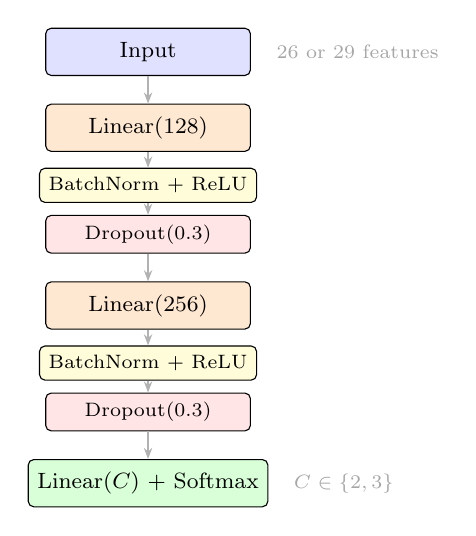
\begin{tikzpicture}[
    node distance=0.35cm,
    layer/.style={draw, rounded corners=2pt, minimum width=2.6cm, minimum height=0.6cm,
                  align=center, font=\footnotesize},
    inp/.style={layer, fill=blue!12},
    hidden/.style={layer, fill=orange!18},
    norm/.style={layer, fill=yellow!15, minimum height=0.4cm, font=\scriptsize},
    drop/.style={layer, fill=red!10, minimum height=0.4cm, font=\scriptsize},
    outp/.style={layer, fill=green!15},
    arr/.style={-{Stealth[length=4pt]}, thick, gray!60},
    ann/.style={font=\scriptsize, text=gray!70, anchor=west},
]

\node[inp] (input) {Input};
\node[ann] at (input.east) [right=0.2cm] {26 or 29 features};

\node[hidden, below=of input] (fc1) {Linear(128)};
\node[norm, below=0.2cm of fc1] (bn1) {BatchNorm + ReLU};
\node[drop, below=0.15cm of bn1] (d1) {Dropout(0.3)};

\node[hidden, below=0.35cm of d1] (fc2) {Linear(256)};
\node[norm, below=0.2cm of fc2] (bn2) {BatchNorm + ReLU};
\node[drop, below=0.15cm of bn2] (d2) {Dropout(0.3)};

\node[outp, below=0.35cm of d2] (outnode) {Linear($C$) + Softmax};
\node[ann] at (outnode.east) [right=0.2cm] {$C \in \{2, 3\}$};

\draw[arr] (input) -- (fc1);
\draw[arr] (fc1) -- (bn1);
\draw[arr] (bn1) -- (d1);
\draw[arr] (d1) -- (fc2);
\draw[arr] (fc2) -- (bn2);
\draw[arr] (bn2) -- (d2);
\draw[arr] (d2) -- (outnode);

\end{tikzpicture}
\caption{StressNet MLP architecture for tabular classification on engineered window features. Two hidden layers with BatchNorm and dropout regularise against overfitting on the small (1\,178-window) dataset.}
\label{fig:arch-mlp}
\end{figure}

\subsection{Part B: Sequence Classification on Raw Time-Series (Baseline)}

\subsubsection{Standalone GRU and LSTM}
Raw wrist signals (6 channels resampled to 4\,Hz) are segmented into 30-second non-overlapping windows ($120 \times 6$).
A GRU or LSTM processes the sequence and the final hidden state is passed to a linear classifier:
\begin{align}
\mathbf{h}_t &= \text{GRU/LSTM}(\mathbf{x}_t, \mathbf{h}_{t-1}) \\
\hat{y} &= \text{softmax}(\mathbf{W} \mathbf{h}_T + \mathbf{b})
\end{align}
These serve as baselines for end-to-end learning from raw signals.

\subsubsection{Standalone 1D-ResNet}
A residual convolutional network processes the window in parallel using three residual blocks (two Conv1d layers with skip connections each), followed by global average pooling and a classification head.
The skip connections address vanishing gradients and enable deeper networks:
\begin{equation}
\mathbf{y} = \text{ReLU}(\mathbf{x} + \mathcal{F}(\mathbf{x}))
\end{equation}

\subsection{Part C: Improved Hybrid Architectures on Raw Time-Series}

Based on EDA insights (inter-subject variability, multi-scale temporal patterns) and literature evidence, we implement five improved architectures with two key preprocessing changes:
\begin{itemize}    \item \textbf{Per-subject z-normalisation}: each subject's signals are z-normalised per channel before windowing, reducing inter-subject scale differences identified in the PCA analysis.
    \item \textbf{60-second overlapping windows} (50\% overlap): longer windows capture more temporal context, and overlap increases training data and captures state transitions.
\end{itemize}

\subsubsection{CNN-LSTM}
A two-layer 1D-CNN front-end (kernels of size 7 and 5, BatchNorm, ReLU, MaxPool) extracts local temporal features, then an LSTM processes the resulting compressed sequence.
The CNN captures short-range patterns (heartbeat morphology in BVP, phasic bursts in EDA) while the LSTM models longer-range temporal dependencies:
\begin{align}
\mathbf{z}_t &= \text{CNN}(\mathbf{x})_t \\
\mathbf{h}_t &= \text{LSTM}(\mathbf{z}_t, \mathbf{h}_{t-1}) \\
\hat{y} &= \text{softmax}(\mathbf{W} \mathbf{h}_T + \mathbf{b})
\end{align}

\subsubsection{CNN-GRU}
Identical architecture but replaces the LSTM with a GRU, which has fewer parameters and often achieves comparable performance.

\subsubsection{CNN-LSTM with Self-Attention}
Adds a learned self-attention layer after the LSTM.
Instead of relying solely on the last hidden state, attention computes a weighted average over all LSTM outputs:
\begin{align}
\alpha_t &= \frac{\exp(\mathbf{v}^\top \mathbf{h}_t)}{\sum_{j} \exp(\mathbf{v}^\top \mathbf{h}_j)} \\
\mathbf{c} &= \sum_t \alpha_t \mathbf{h}_t
\end{align}
This allows the model to focus on the most informative time steps rather than compressing all information into the final state.

% --- CNN-LSTM-ATTENTION ARCHITECTURE FIGURE ---
\begin{figure}[H]
\centering
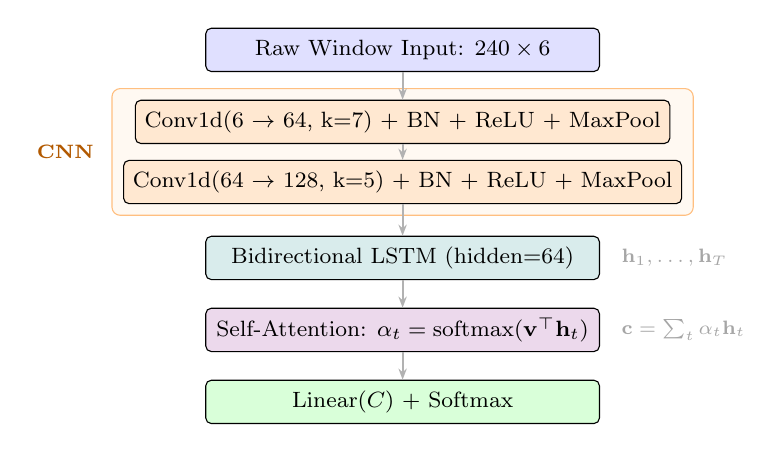
\begin{tikzpicture}[
    node distance=0.3cm,
    layer/.style={draw, rounded corners=2pt, minimum height=0.55cm,
                  align=center, font=\footnotesize},
    inp/.style={layer, fill=blue!12, minimum width=5.0cm},
    conv/.style={layer, fill=orange!18, minimum width=5.0cm},
    rnn/.style={layer, fill=teal!15, minimum width=5.0cm},
    attn/.style={layer, fill=violet!15, minimum width=5.0cm},
    outp/.style={layer, fill=green!15, minimum width=5.0cm},
    pool/.style={layer, fill=yellow!12, minimum width=5.0cm, minimum height=0.4cm, font=\scriptsize},
    arr/.style={-{Stealth[length=4pt]}, thick, gray!60},
    ann/.style={font=\scriptsize, text=gray!70, anchor=west},
    brace/.style={decorate, decoration={brace, amplitude=5pt}},
]

\node[inp] (input) {Raw Window Input: $240 \times 6$};

% CNN block
\node[conv, below=0.35cm of input] (c1) {Conv1d(6 $\to$ 64, k=7) + BN + ReLU + MaxPool};
\node[conv, below=0.2cm of c1] (c2) {Conv1d(64 $\to$ 128, k=5) + BN + ReLU + MaxPool};

% Annotation brace for CNN
\begin{scope}[on background layer]
\node[draw=orange!50, fill=orange!5, rounded corners=3pt,
      fit=(c1)(c2), inner xsep=4pt, inner ysep=4pt] (cnnbox) {};
\end{scope}
\node[font=\scriptsize\bfseries, text=orange!70!black, anchor=east] at (cnnbox.west) [left=0.1cm] {CNN};

% LSTM
\node[rnn, below=0.4cm of c2] (lstm) {Bidirectional LSTM (hidden=64)};
\node[ann] at (lstm.east) [right=0.15cm] {$\mathbf{h}_1, \ldots, \mathbf{h}_T$};

% Self-attention
\node[attn, below=0.35cm of lstm] (att) {Self-Attention: $\alpha_t = \mathrm{softmax}(\mathbf{v}^\top\mathbf{h}_t)$};
\node[ann] at (att.east) [right=0.15cm] {$\mathbf{c} = \sum_t \alpha_t \mathbf{h}_t$};

% Output
\node[outp, below=0.35cm of att] (outnode) {Linear($C$) + Softmax};

% Arrows
\draw[arr] (input) -- (c1);
\draw[arr] (c1) -- (c2);
\draw[arr] (c2) -- (lstm);
\draw[arr] (lstm) -- (att);
\draw[arr] (att) -- (outnode);

\end{tikzpicture}
\caption{CNN-LSTM with self-attention architecture. Two convolutional layers extract local temporal features from raw 60-second windows, an LSTM captures long-range dependencies across the compressed sequence, and a learned attention mechanism weights the most informative time steps for classification. This architecture achieves the best binary Macro-F1 (0.897) among all raw-signal models.}
\label{fig:arch-cnn-lstm-attn}
\end{figure}

\subsubsection{Multi-Scale CNN-LSTM}
Parallel 1D convolutions with kernel sizes 3, 7, and 15 capture patterns at different temporal scales simultaneously---fast BVP oscillations (kernel~3), moderate EDA dynamics (kernel~7), and slow temperature drift (kernel~15).
Outputs are concatenated, pooled, then fed to an LSTM with self-attention.

\subsubsection{ResNet-LSTM}
Three residual blocks serve as the CNN front-end (benefiting from skip connections for training stability), followed by an LSTM and self-attention back-end.
This combines the depth-stability of residual learning with temporal modelling.

% --- RESNET-LSTM ARCHITECTURE FIGURE ---
\begin{figure}[H]
\centering
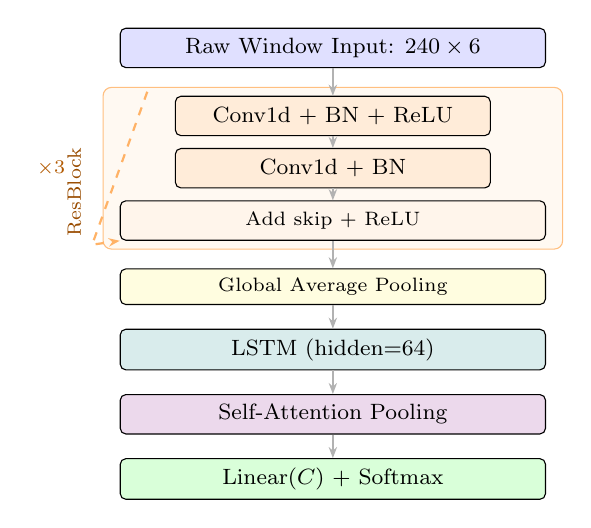
\begin{tikzpicture}[
    node distance=0.3cm,
    layer/.style={draw, rounded corners=2pt, minimum height=0.5cm,
                  align=center, font=\footnotesize},
    inp/.style={layer, fill=blue!12, minimum width=5.4cm},
    res/.style={layer, fill=orange!15, minimum width=4.0cm},
    rnn/.style={layer, fill=teal!15, minimum width=5.4cm},
    attn/.style={layer, fill=violet!15, minimum width=5.4cm},
    outp/.style={layer, fill=green!15, minimum width=5.4cm},
    pool/.style={layer, fill=yellow!12, minimum width=5.4cm, minimum height=0.4cm, font=\scriptsize},
    arr/.style={-{Stealth[length=4pt]}, thick, gray!60},
    skip/.style={-{Stealth[length=4pt]}, thick, orange!60, dashed},
    ann/.style={font=\scriptsize, text=gray!70, anchor=west},
]

\node[inp] (input) {Raw Window Input: $240 \times 6$};

% ResBlock 1
\node[res, below=0.35cm of input] (rb1a) {Conv1d + BN + ReLU};
\node[res, below=0.15cm of rb1a] (rb1b) {Conv1d + BN};
\node[layer, fill=orange!8, minimum width=5.4cm, below=0.15cm of rb1b, font=\scriptsize] (rb1add) {Add skip + ReLU};

% Skip connection for block 1
\draw[arr] (rb1a) -- (rb1b);
\draw[arr] (rb1b) -- (rb1add);
\draw[skip] ($(rb1a.north west)+(-0.35, 0.05)$) -- ($(rb1add.south west)+(-0.35, -0.05)$)
    -- (rb1add.south west);
\draw[arr] (input) -- (rb1a);

% Brace for res blocks
\begin{scope}[on background layer]
\node[draw=orange!50, fill=orange!5, rounded corners=3pt,
      fit=(rb1a)(rb1b)(rb1add), inner xsep=6pt, inner ysep=3pt] (resbox1) {};
\end{scope}
\node[font=\scriptsize\bfseries, text=orange!70!black, anchor=east] at (resbox1.west) [left=0.35cm] {$\times 3$};
\node[font=\scriptsize, text=orange!60!black, anchor=east] at (resbox1.west) [left=0.15cm, yshift=-0.3cm] {\rotatebox{90}{ResBlock}};

% Global avg pool
\node[pool, below=0.35cm of rb1add] (gap) {Global Average Pooling};
\draw[arr] (rb1add) -- (gap);

% LSTM
\node[rnn, below=0.3cm of gap] (lstm) {LSTM (hidden=64)};
\draw[arr] (gap) -- (lstm);

% Attention
\node[attn, below=0.3cm of lstm] (att) {Self-Attention Pooling};
\draw[arr] (lstm) -- (att);

% Output
\node[outp, below=0.3cm of att] (outnode) {Linear($C$) + Softmax};
\draw[arr] (att) -- (outnode);

\end{tikzpicture}
\caption{ResNet-LSTM architecture. Three residual blocks (each with two Conv1d layers and a skip connection) provide a deep, gradient-stable feature extractor. Global average pooling compresses the spatial dimension before feeding into an LSTM with self-attention. This architecture achieves the best 3-class Macro-F1 (0.667) among raw-signal models.}
\label{fig:arch-resnet-lstm}
\end{figure}


% ======================================================================
\section{Results}
\label{sec:results}
% ======================================================================

\subsection{Part A: Tabular Classification Results}

\subsubsection{3-Class Classification}

\begin{table}[H]
\centering
\caption{3-class LOSO results on engineered features. Best values in \textbf{bold}.}
\label{tab:3class}
\begin{tabular}{llcc}
\toprule
\textbf{Model} & \textbf{Data Variant} & \textbf{Mean Accuracy} & \textbf{Mean Macro-F1} \\
\midrule
Logistic Regression & sensor        & $0.719 \pm 0.172$ & $0.588 \pm 0.180$ \\
Logistic Regression & sensor+demo   & $0.718 \pm 0.167$ & $0.607 \pm 0.181$ \\
\midrule
Random Forest       & sensor        & $0.731 \pm 0.205$ & $0.663 \pm 0.230$ \\
Random Forest       & sensor+demo   & $0.737 \pm 0.194$ & $0.664 \pm 0.223$ \\
\midrule
XGBoost             & sensor        & $0.737 \pm 0.205$ & $\mathbf{0.677 \pm 0.235}$ \\
XGBoost             & sensor+demo   & $\mathbf{0.742 \pm 0.192}$ & $0.663 \pm 0.223$ \\
\midrule
MLP (StressNet)     & sensor        & $0.723 \pm 0.164$ & $0.688 \pm 0.182$ \\
MLP (StressNet)     & sensor+demo   & $0.677 \pm 0.137$ & $0.619 \pm 0.146$ \\
\bottomrule
\end{tabular}
\end{table}

\begin{table}[H]
\centering
\caption{Per-class metrics for 3-class experiments (aggregated across all LOSO folds).}
\label{tab:3class-perclass}
\begin{tabular}{llccc}
\toprule
\textbf{Model} & \textbf{Class} & \textbf{Precision} & \textbf{Recall} & \textbf{F1} \\
\midrule
Logistic Regression & Amusement & 0.410 & 0.221 & 0.287 \\
Logistic Regression & Baseline  & 0.723 & 0.817 & 0.767 \\
Logistic Regression & Stress    & 0.799 & 0.817 & 0.808 \\
\midrule
Random Forest       & Amusement & 0.550 & 0.508 & 0.528 \\
Random Forest       & Baseline  & 0.773 & 0.748 & 0.761 \\
Random Forest       & Stress    & 0.749 & 0.823 & 0.784 \\
\midrule
XGBoost             & Amusement & 0.573 & 0.523 & 0.547 \\
XGBoost             & Baseline  & 0.783 & 0.748 & 0.765 \\
XGBoost             & Stress    & 0.738 & 0.831 & 0.781 \\
\midrule
MLP (StressNet)     & Amusement & 0.405 & 0.636 & 0.495 \\
MLP (StressNet)     & Baseline  & 0.863 & 0.624 & 0.725 \\
MLP (StressNet)     & Stress    & 0.804 & 0.946 & 0.869 \\
\bottomrule
\end{tabular}
\end{table}

\begin{table}[H]
\centering
\caption{MLP per-subject LOSO accuracy for 3-class classification (sensor features).}
\label{tab:mlp-persub-3class}
\small
\begin{tabular}{lccccccccccccccc}
\toprule
& S2 & S3 & S4 & S5 & S6 & S7 & S8 & S9 & S10 & S11 & S13 & S14 & S15 & S16 & S17 \\
\midrule
Acc & .71 & .56 & .49 & .79 & .77 & .74 & .72 & .94 & .72 & .94 & .79 & .42 & .89 & .89 & .51 \\
F1  & .72 & .53 & .50 & .76 & .76 & .74 & .72 & .92 & .68 & .92 & .61 & .31 & .87 & .86 & .42 \\
\bottomrule
\end{tabular}
\end{table}

Amusement is the hardest class across all models (F1 $\leq$ 0.55 for tree models, 0.29 for Logistic Regression), as expected given its small sample size and physiological overlap with Baseline.
XGBoost achieves the highest 3-class Macro-F1 (0.677 on sensor features) and highest accuracy (0.742 with demographics).
The MLP achieves competitive Macro-F1 (0.688) with the \textbf{lowest fold-to-fold variance} ($\pm$0.164), indicating more stable generalisation, and the highest Stress F1 (0.869).
Demographics provide marginal benefit for tree models ($<$1\%) and hurt MLP performance, likely because subject-constant features risk acting as identifiers rather than genuine predictors.
Per-subject results (Table~\ref{tab:mlp-persub-3class}) reveal large variance: S9 and S11 achieve $>$0.93 accuracy while S14 and S17 fall below 0.51, reflecting genuine inter-subject physiological differences.

\begin{figure}[H]
\centering
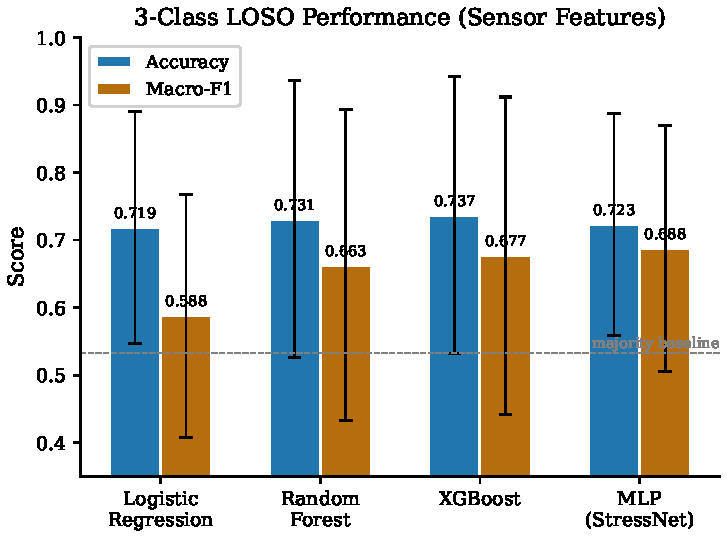
\includegraphics[width=0.78\linewidth]{tabular_3class_comparison.pdf}
\caption{Mean LOSO accuracy and Macro-F1 ($\pm$1 SD) for all tabular models on the 3-class task (sensor features only). XGBoost achieves the highest Macro-F1 (0.677) and the MLP the lowest fold-to-fold variance. The dashed line marks the majority-class baseline (53.3\%).}
\label{fig:tabular-3class}
\end{figure}

\begin{figure}[H]
\centering
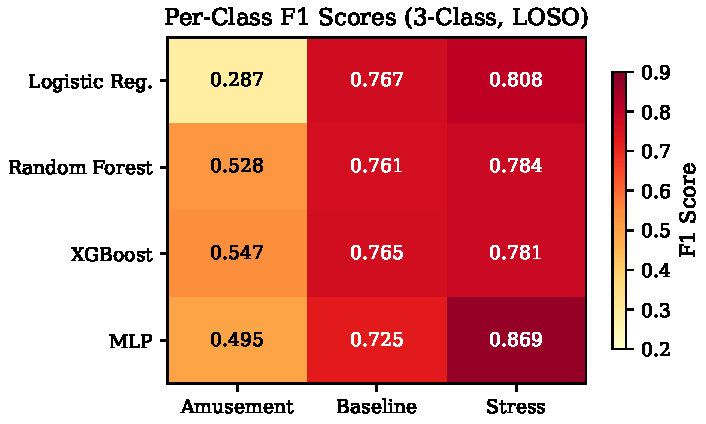
\includegraphics[width=0.65\linewidth]{tabular_3class_perclass_f1.pdf}
\caption{Per-class F1 scores for all tabular models on the 3-class task. Amusement is consistently the hardest class (F1 $\leq$ 0.55), reflecting its small sample size and physiological overlap with Baseline. The MLP achieves the highest Stress F1 (0.869).}
\label{fig:tabular-3class-perclass}
\end{figure}

\subsubsection{Binary Classification (Stress vs.\ Not-Stress)}

\begin{table}[H]
\centering
\caption{Binary LOSO results on engineered features. Best values in \textbf{bold}.}
\label{tab:binary}
\begin{tabular}{llcc}
\toprule
\textbf{Model} & \textbf{Data Variant} & \textbf{Mean Accuracy} & \textbf{Mean Macro-F1} \\
\midrule
Logistic Regression & sensor        & $0.886 \pm 0.161$ & $0.866 \pm 0.188$ \\
Logistic Regression & sensor+demo   & $0.873 \pm 0.162$ & $0.853 \pm 0.177$ \\
\midrule
Random Forest       & sensor        & $0.865 \pm 0.214$ & $0.837 \pm 0.244$ \\
Random Forest       & sensor+demo   & $0.878 \pm 0.205$ & $0.851 \pm 0.238$ \\
\midrule
XGBoost             & sensor        & $0.858 \pm 0.219$ & $0.835 \pm 0.239$ \\
XGBoost             & sensor+demo   & $0.867 \pm 0.205$ & $0.845 \pm 0.228$ \\
\midrule
MLP (StressNet)     & sensor        & $0.897 \pm 0.190$ & $0.893 \pm 0.192$ \\
MLP (StressNet)     & sensor+demo   & $\mathbf{0.928 \pm 0.118}$ & $\mathbf{0.921 \pm 0.123}$ \\
\bottomrule
\end{tabular}
\end{table}

\begin{table}[H]
\centering
\caption{Per-class metrics for binary experiments (aggregated across LOSO folds).}
\label{tab:binary-perclass}
\begin{tabular}{llccc}
\toprule
\textbf{Model} & \textbf{Class} & \textbf{Precision} & \textbf{Recall} & \textbf{F1} \\
\midrule
Logistic Regression & Not-Stress & 0.914 & 0.922 & 0.918 \\
Logistic Regression & Stress     & 0.816 & 0.800 & 0.808 \\
\midrule
Random Forest       & Not-Stress & 0.911 & 0.893 & 0.902 \\
Random Forest       & Stress     & 0.763 & 0.797 & 0.780 \\
\midrule
XGBoost             & Not-Stress & 0.913 & 0.880 & 0.896 \\
XGBoost             & Stress     & 0.743 & 0.806 & 0.773 \\
\midrule
MLP (sensor)        & Not-Stress & 0.974 & 0.875 & 0.922 \\
MLP (sensor)        & Stress     & 0.765 & 0.946 & 0.846 \\
\midrule
MLP (sensor+demo)   & Not-Stress & 0.969 & 0.926 & 0.947 \\
MLP (sensor+demo)   & Stress     & 0.844 & 0.932 & 0.886 \\
\bottomrule
\end{tabular}
\end{table}

\begin{table}[H]
\centering
\caption{MLP per-subject LOSO accuracy for binary classification (sensor+demographics).}
\label{tab:mlp-persub-binary}
\small
\begin{tabular}{lccccccccccccccc}
\toprule
& S2 & S3 & S4 & S5 & S6 & S7 & S8 & S9 & S10 & S11 & S13 & S14 & S15 & S16 & S17 \\
\midrule
Acc & .99 & .65 & .99 & .99 & 1.0 & .97 & .98 & 1.0 & 1.0 & .87 & 1.0 & .70 & .99 & 1.0 & .80 \\
F1  & .98 & .64 & .98 & .98 & 1.0 & .97 & .97 & 1.0 & 1.0 & .83 & 1.0 & .69 & .99 & 1.0 & .77 \\
\bottomrule
\end{tabular}
\end{table}

The MLP is the clear winner for binary stress detection.
With sensor+demographics, it achieves the highest accuracy ($0.928 \pm 0.118$) and Macro-F1 ($0.921 \pm 0.123$), with 93.2\% Stress recall and the lowest fold-to-fold variance.
Even with sensor-only features, the MLP reaches 0.897 accuracy and 0.893 F1, with 94.6\% Stress recall.
Logistic Regression provides a strong linear baseline (0.886 accuracy), outperforming both tree ensembles and suggesting that Stress vs.\ Not-Stress is largely linearly separable.
All models gain 12--19 percentage points in Macro-F1 moving from 3-class to binary, confirming that the Amusement/Baseline distinction drives most of the classification difficulty.

\begin{figure}[H]
\centering
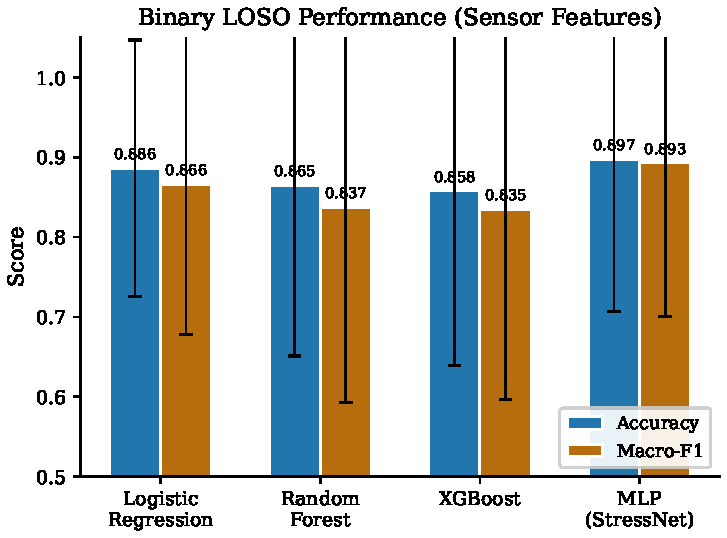
\includegraphics[width=0.78\linewidth]{tabular_binary_comparison.pdf}
\caption{Mean LOSO accuracy and Macro-F1 ($\pm$1 SD) for all tabular models on the binary (Stress vs.\ Not-Stress) task. The MLP achieves the highest scores (Accuracy = 0.897, Macro-F1 = 0.893 on sensor features). All models gain 12--19 pp in F1 relative to the 3-class task.}
\label{fig:tabular-binary}
\end{figure}

\begin{figure}[H]
\centering
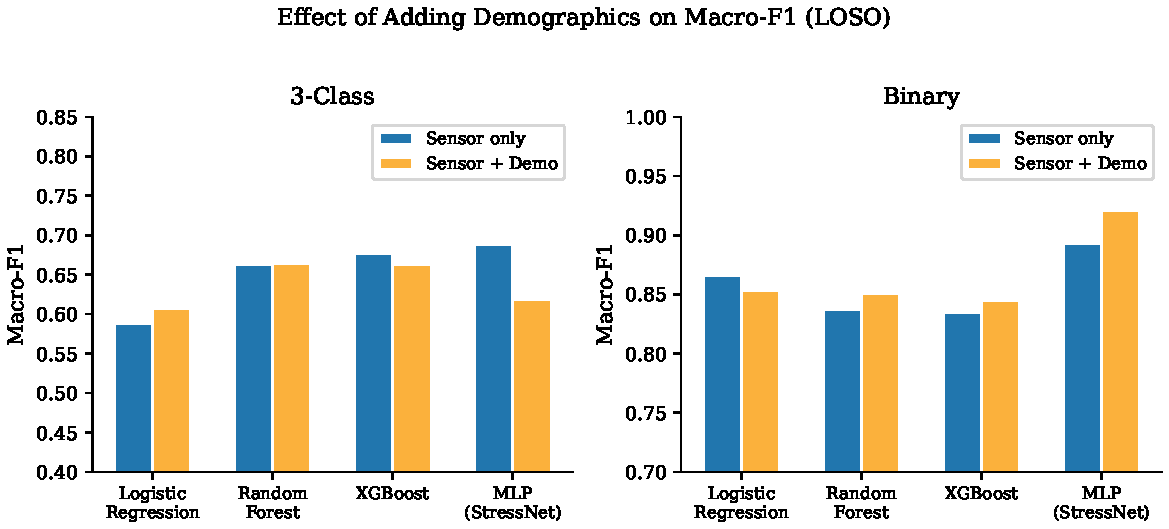
\includegraphics[width=0.65\linewidth]{sensor_vs_demo_impact.pdf}
\caption{Effect of adding demographic features on Macro-F1 for each tabular model. Demographics provide marginal benefit for tree ensembles ($<$1\%) and a substantial boost for the binary MLP (+2.8 pp), but hurt the 3-class MLP, suggesting subject-constant features risk acting as identifiers.}
\label{fig:sensor-vs-demo}
\end{figure}

\begin{figure}[H]
\centering
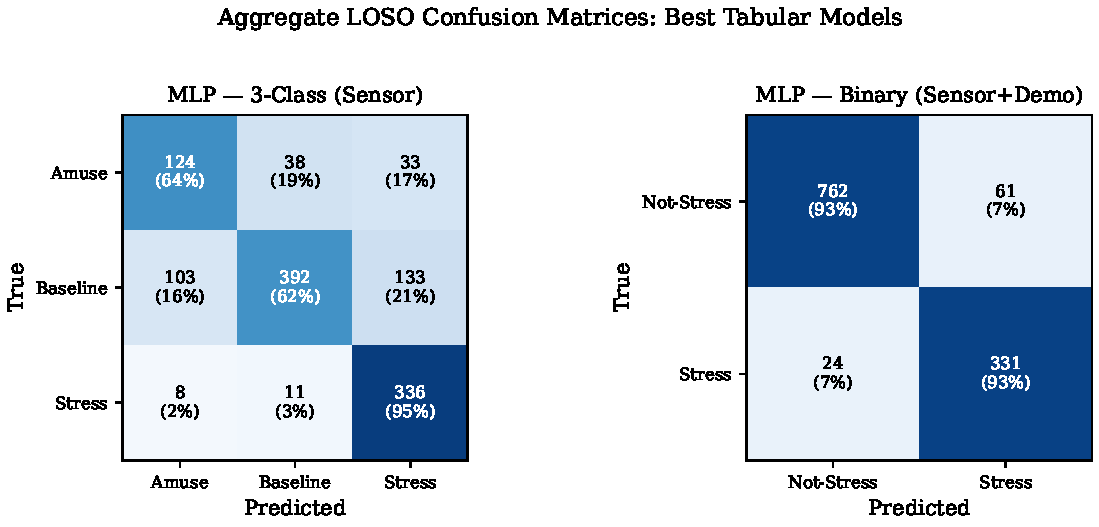
\includegraphics[width=0.85\linewidth]{tabular_confusion_matrices.pdf}
\caption{Aggregate LOSO confusion matrices for the best tabular models. \textbf{Left}: MLP on the 3-class task (sensor features)---Stress recall is high (94.6\%) but Amusement is frequently confused with Baseline. \textbf{Right}: MLP on the binary task (sensor+demographics)---92.6\% of Not-Stress and 93.2\% of Stress windows are correctly classified.}
\label{fig:tabular-cm}
\end{figure}

\begin{figure}[H]
\centering
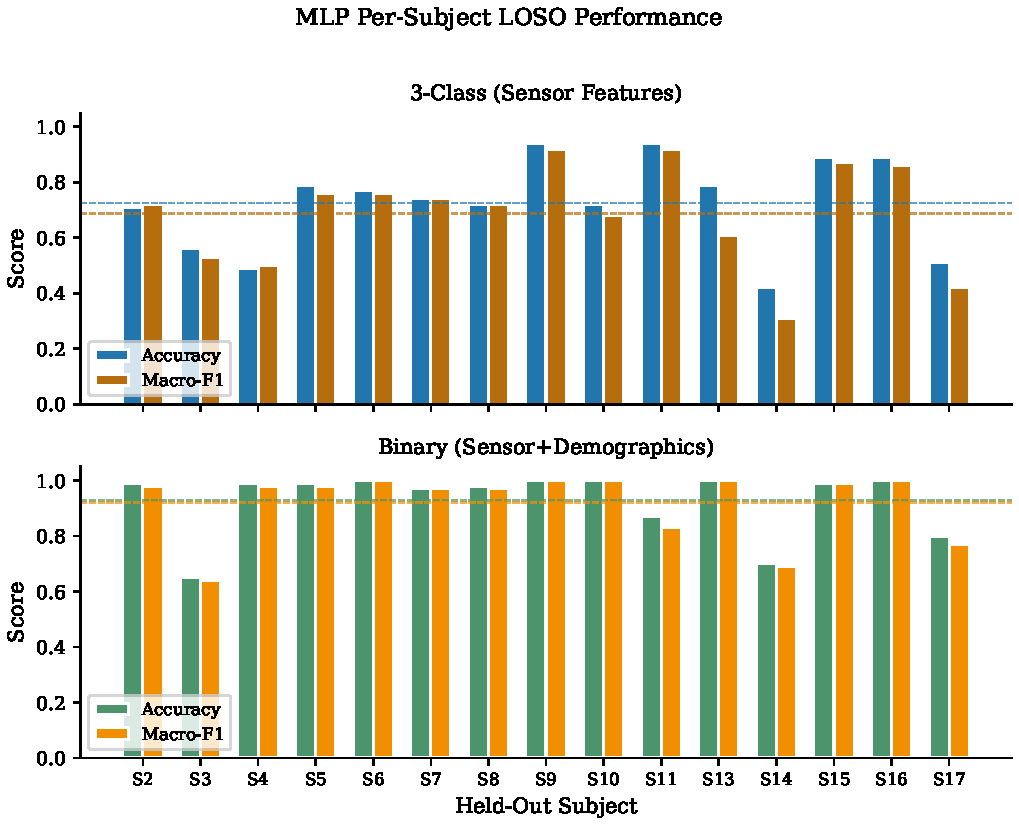
\includegraphics[width=0.85\linewidth]{mlp_per_subject_loso.pdf}
\caption{MLP per-subject LOSO performance. \textbf{Top}: 3-class (sensor features)---S9 and S11 achieve $>$0.92 accuracy while S14 and S17 fall below 0.51. \textbf{Bottom}: binary (sensor+demographics)---most subjects reach near-perfect accuracy, but S3, S14, and S17 remain harder. Dashed lines show cross-subject means.}
\label{fig:mlp-persub}
\end{figure}

\subsection{Part B: Baseline Deep Sequence Models}

\begin{table}[H]
\centering
\caption{Baseline RNN and ResNet results on 30s non-overlapping raw windows (LOSO).}
\label{tab:baseline-seq}
\begin{tabular}{lcc}
\toprule
\textbf{Model} & \textbf{Mean Accuracy} & \textbf{Mean Macro-F1} \\
\midrule
GRU (3-class)    & $0.612 \pm 0.171$ & $0.519 \pm 0.172$ \\
LSTM (3-class)   & $0.500 \pm 0.235$ & $0.409 \pm 0.203$ \\
ResNet (3-class) & $0.588 \pm 0.158$ & $0.494 \pm 0.163$ \\
\midrule
GRU (binary)     & $0.740 \pm 0.162$ & $0.688 \pm 0.185$ \\
LSTM (binary)    & $0.763 \pm 0.193$ & $0.690 \pm 0.238$ \\
ResNet (binary)  & $0.794 \pm 0.127$ & $0.738 \pm 0.165$ \\
\bottomrule
\end{tabular}
\end{table}

\begin{table}[H]
\centering
\caption{Per-class metrics for baseline sequence models (aggregated across LOSO folds).}
\label{tab:baseline-seq-perclass}
\begin{tabular}{llccc}
\toprule
\textbf{Model} & \textbf{Class} & \textbf{Precision} & \textbf{Recall} & \textbf{F1} \\
\midrule
GRU (3-class)    & Amusement  & 0.384 & 0.384 & 0.384 \\
GRU (3-class)    & Baseline   & 0.721 & 0.676 & 0.698 \\
GRU (3-class)    & Stress     & 0.567 & 0.630 & 0.597 \\
\midrule
LSTM (3-class)   & Amusement  & 0.181 & 0.319 & 0.231 \\
LSTM (3-class)   & Baseline   & 0.756 & 0.534 & 0.626 \\
LSTM (3-class)   & Stress     & 0.495 & 0.540 & 0.516 \\
\midrule
ResNet (3-class) & Amusement  & 0.225 & 0.270 & 0.246 \\
ResNet (3-class) & Baseline   & 0.693 & 0.616 & 0.652 \\
ResNet (3-class) & Stress     & 0.661 & 0.716 & 0.688 \\
\bottomrule
\end{tabular}
\end{table}

\begin{table}[H]
\centering
\caption{GRU per-subject LOSO accuracy for 3-class classification on raw signals.}
\label{tab:gru-persub}
\small
\begin{tabular}{lccccccccccccccc}
\toprule
& S2 & S3 & S4 & S5 & S6 & S7 & S8 & S9 & S10 & S11 & S13 & S14 & S15 & S16 & S17 \\
\midrule
Acc & .66 & .38 & .85 & .53 & .68 & .57 & .24 & .64 & .84 & .66 & .78 & .42 & .73 & .53 & .68 \\
F1  & .53 & .30 & .72 & .35 & .68 & .42 & .20 & .45 & .82 & .55 & .58 & .42 & .73 & .53 & .51 \\
\bottomrule
\end{tabular}
\end{table}

Standalone RNNs and ResNets on raw 30-second, non-overlapping windows achieve 0.50--0.79 accuracy---substantially below the tabular models.
The GRU is the best-performing RNN (3-class Macro-F1 = 0.519), but even it falls far short of the tabular XGBoost (0.677).
Per-subject results (Table~\ref{tab:gru-persub}) show extreme variance: S10 achieves 0.84 while S8 drops to 0.24.
This under-performance is attributable to (a)~the very low wrist sampling rate (4\,Hz effective); (b)~large inter-subject variability without per-subject normalisation; and (c)~insufficient training data from non-overlapping segmentation.

\begin{figure}[H]
\centering
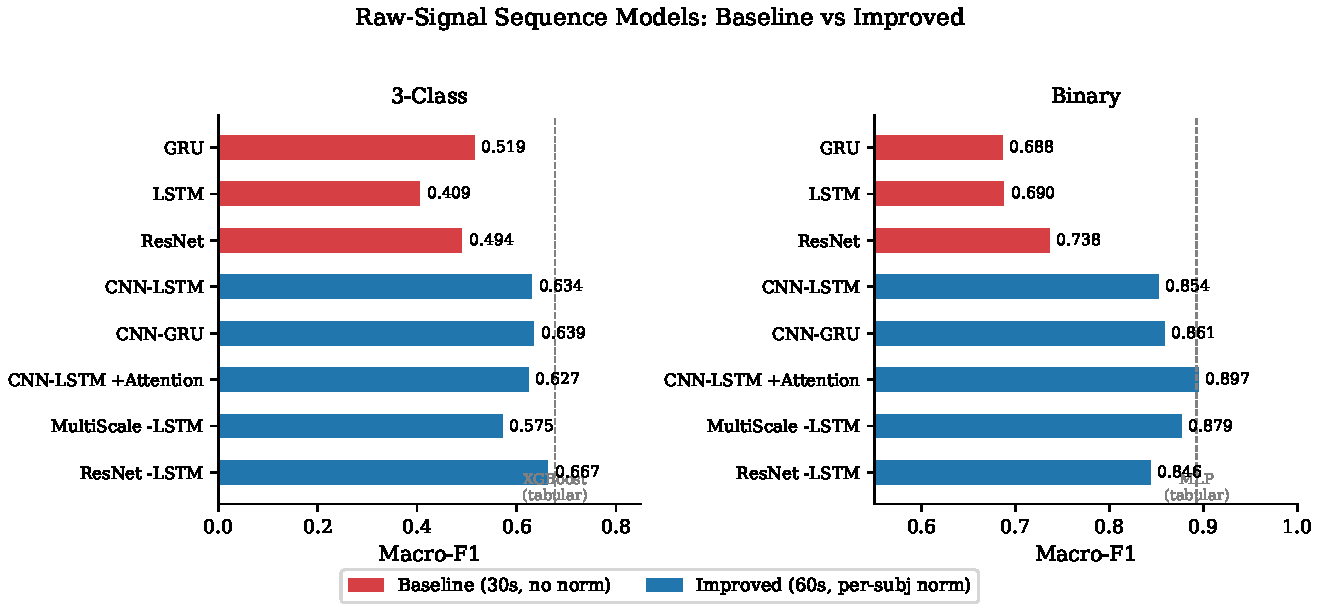
\includegraphics[width=0.95\linewidth]{raw_signal_baseline_vs_improved.pdf}
\caption{Macro-F1 comparison of all raw-signal sequence models. \textcolor{red!70!black}{Red} bars show baseline models (30s non-overlapping windows, no per-subject normalisation); \textcolor{blue!70!black}{blue} bars show improved models (60s overlapping windows, per-subject z-normalisation). Dashed vertical lines mark the best tabular model in each task for reference. The improved pipeline closes most of the gap between raw-signal and engineered-feature performance.}
\label{fig:raw-baseline-vs-improved}
\end{figure}

\subsection{Part C: Improved Hybrid Models}

The improved pipeline (per-subject normalisation, 60s overlapping windows, hybrid architectures) addresses all three limitations of the baseline sequence models.
Five architectures are compared under identical LOSO evaluation:

\begin{table}[H]
\centering
\caption{Improved hybrid model results on 60s overlapping raw windows (LOSO). Best values in \textbf{bold}.}
\label{tab:improved}
\begin{tabular}{lcccc}
\toprule
 & \multicolumn{2}{c}{\textbf{3-Class}} & \multicolumn{2}{c}{\textbf{Binary}} \\
\cmidrule(lr){2-3} \cmidrule(lr){4-5}
\textbf{Model} & \textbf{Acc} & \textbf{F1} & \textbf{Acc} & \textbf{F1} \\
\midrule
CNN-LSTM            & $0.693 \pm 0.177$ & $0.634 \pm 0.190$ & $0.881 \pm 0.169$ & $0.854 \pm 0.206$ \\
CNN-GRU             & $0.702 \pm 0.175$ & $0.639 \pm 0.193$ & $0.885 \pm 0.178$ & $0.861 \pm 0.210$ \\
CNN-LSTM-Attention  & $0.703 \pm 0.176$ & $0.627 \pm 0.187$ & $\mathbf{0.908 \pm 0.131}$ & $\mathbf{0.897 \pm 0.145}$ \\
MultiScale-LSTM     & $0.651 \pm 0.160$ & $0.575 \pm 0.146$ & $0.899 \pm 0.167$ & $0.879 \pm 0.190$ \\
ResNet-LSTM         & $\mathbf{0.731 \pm 0.155}$ & $\mathbf{0.667 \pm 0.180}$ & $0.866 \pm 0.170$ & $0.846 \pm 0.187$ \\
\bottomrule
\end{tabular}
\end{table}

\begin{table}[H]
\centering
\caption{Per-class metrics for improved hybrid models (3-class, aggregated across LOSO folds).}
\label{tab:hybrid-3class-perclass}
\begin{tabular}{llccc}
\toprule
\textbf{Model} & \textbf{Class} & \textbf{Precision} & \textbf{Recall} & \textbf{F1} \\
\midrule
CNN-LSTM           & Amusement & 0.347 & 0.414 & 0.377 \\
CNN-LSTM           & Baseline  & 0.785 & 0.709 & 0.745 \\
CNN-LSTM           & Stress    & 0.771 & 0.819 & 0.794 \\
\midrule
CNN-GRU            & Amusement & 0.311 & 0.371 & 0.338 \\
CNN-GRU            & Baseline  & 0.777 & 0.736 & 0.756 \\
CNN-GRU            & Stress    & 0.838 & 0.825 & 0.832 \\
\midrule
CNN-LSTM-Attention & Amusement & 0.333 & 0.371 & 0.351 \\
CNN-LSTM-Attention & Baseline  & 0.796 & 0.738 & 0.766 \\
CNN-LSTM-Attention & Stress    & 0.774 & 0.825 & 0.799 \\
\midrule
MultiScale-LSTM    & Amusement & 0.210 & 0.269 & 0.236 \\
MultiScale-LSTM    & Baseline  & 0.716 & 0.680 & 0.698 \\
MultiScale-LSTM    & Stress    & 0.871 & 0.813 & 0.841 \\
\midrule
ResNet-LSTM        & Amusement & 0.372 & 0.446 & 0.406 \\
ResNet-LSTM        & Baseline  & 0.813 & 0.748 & 0.779 \\
ResNet-LSTM        & Stress    & 0.833 & 0.858 & 0.846 \\
\bottomrule
\end{tabular}
\end{table}

\begin{table}[H]
\centering
\caption{Per-class metrics for improved hybrid models (binary, aggregated across LOSO folds).}
\label{tab:hybrid-binary-perclass}
\begin{tabular}{llccc}
\toprule
\textbf{Model} & \textbf{Class} & \textbf{Precision} & \textbf{Recall} & \textbf{F1} \\
\midrule
CNN-LSTM           & Not-Stress & 0.910 & 0.918 & 0.914 \\
CNN-LSTM           & Stress     & 0.806 & 0.789 & 0.798 \\
\midrule
CNN-GRU            & Not-Stress & 0.911 & 0.924 & 0.917 \\
CNN-GRU            & Stress     & 0.816 & 0.789 & 0.802 \\
\midrule
CNN-LSTM-Attention & Not-Stress & 0.959 & 0.907 & 0.932 \\
CNN-LSTM-Attention & Stress     & 0.807 & 0.910 & 0.856 \\
\midrule
MultiScale-LSTM    & Not-Stress & 0.920 & 0.935 & 0.928 \\
MultiScale-LSTM    & Stress     & 0.843 & 0.810 & 0.826 \\
\midrule
ResNet-LSTM        & Not-Stress & 0.919 & 0.884 & 0.901 \\
ResNet-LSTM        & Stress     & 0.751 & 0.819 & 0.784 \\
\bottomrule
\end{tabular}
\end{table}

\begin{table}[H]
\centering
\caption{CNN-LSTM-Attention per-subject LOSO accuracy for binary classification (best hybrid).}
\label{tab:attention-persub}
\small
\begin{tabular}{lccccccccccccccc}
\toprule
& S2 & S3 & S4 & S5 & S6 & S7 & S8 & S9 & S10 & S11 & S13 & S14 & S15 & S16 & S17 \\
\midrule
Acc & .83 & .60 & 1.0 & .97 & 1.0 & .97 & .95 & 1.0 & 1.0 & .99 & .87 & .71 & 1.0 & 1.0 & .73 \\
F1  & .82 & .56 & 1.0 & .97 & 1.0 & .97 & .94 & 1.0 & 1.0 & .98 & .86 & .66 & 1.0 & 1.0 & .72 \\
\bottomrule
\end{tabular}
\end{table}

\begin{table}[H]
\centering
\caption{ResNet-LSTM per-subject LOSO accuracy for 3-class classification (best hybrid 3-class).}
\label{tab:resnetlstm-persub}
\small
\begin{tabular}{lccccccccccccccc}
\toprule
& S2 & S3 & S4 & S5 & S6 & S7 & S8 & S9 & S10 & S11 & S13 & S14 & S15 & S16 & S17 \\
\midrule
Acc & .92 & .60 & .51 & .77 & .62 & .66 & .89 & 1.0 & .64 & .91 & .65 & .55 & .63 & .90 & .72 \\
F1  & .86 & .59 & .54 & .60 & .52 & .68 & .80 & 1.0 & .61 & .90 & .50 & .38 & .58 & .89 & .56 \\
\bottomrule
\end{tabular}
\end{table}

The hybrid architectures substantially improve over baseline sequence models.
\textbf{ResNet-LSTM} achieves the best 3-class performance (accuracy $0.731$, Macro-F1 $0.667$), closely matching the tabular XGBoost (0.677) and demonstrating that residual convolutional front-ends paired with temporal back-ends can approach hand-crafted feature pipelines.
\textbf{CNN-LSTM-Attention} achieves the best binary performance (accuracy $0.908$, Macro-F1 $0.897$), matching the tabular MLP ($0.921$) and reaching 91.0\% Stress recall through attention-weighted temporal pooling.
The MultiScale-LSTM under-performs, suggesting that the additional capacity from parallel kernel sizes does not compensate for the increased parameter count on this dataset size.

\begin{figure}[H]
\centering
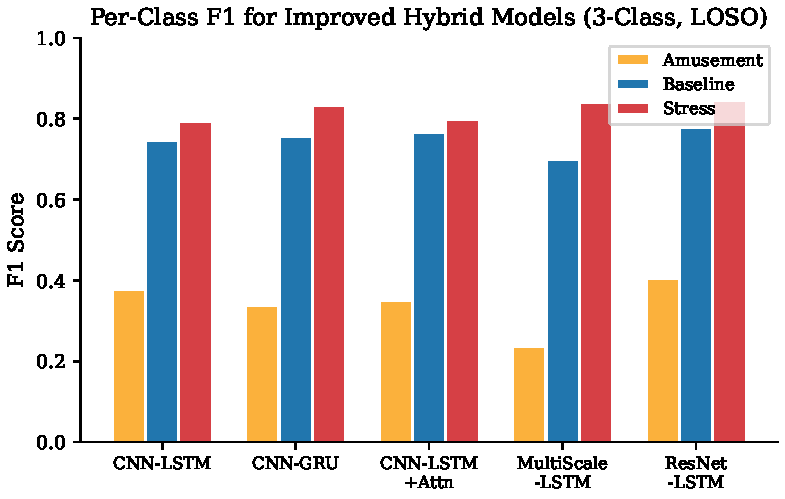
\includegraphics[width=0.78\linewidth]{hybrid_3class_perclass_f1.pdf}
\caption{Per-class F1 for all improved hybrid architectures on the 3-class task. Amusement remains the hardest class across all models. ResNet-LSTM achieves the highest Amusement F1 (0.406) and the best overall balance; MultiScale-LSTM under-performs, suggesting the added capacity from parallel kernels is not justified at this dataset size.}
\label{fig:hybrid-perclass}
\end{figure}

\begin{figure}[H]
\centering
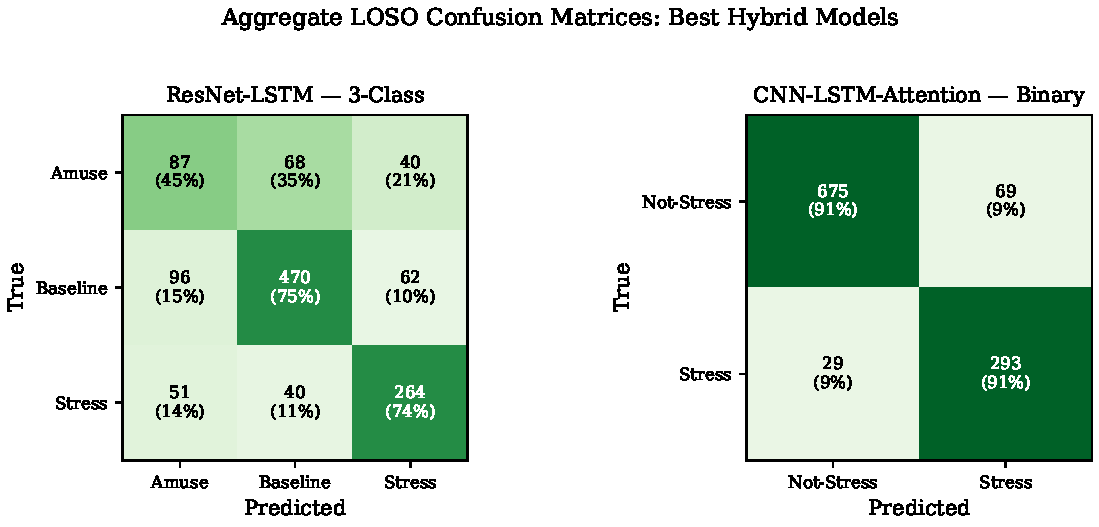
\includegraphics[width=0.85\linewidth]{hybrid_confusion_matrices.pdf}
\caption{Aggregate LOSO confusion matrices for the best hybrid models. \textbf{Left}: ResNet-LSTM on the 3-class task---Amusement confusion with Baseline is reduced relative to tabular models. \textbf{Right}: CNN-LSTM-Attention on the binary task---91.0\% Stress recall with only 9.3\% false-alarm rate on Not-Stress windows.}
\label{fig:hybrid-cm}
\end{figure}

\begin{figure}[H]
\centering
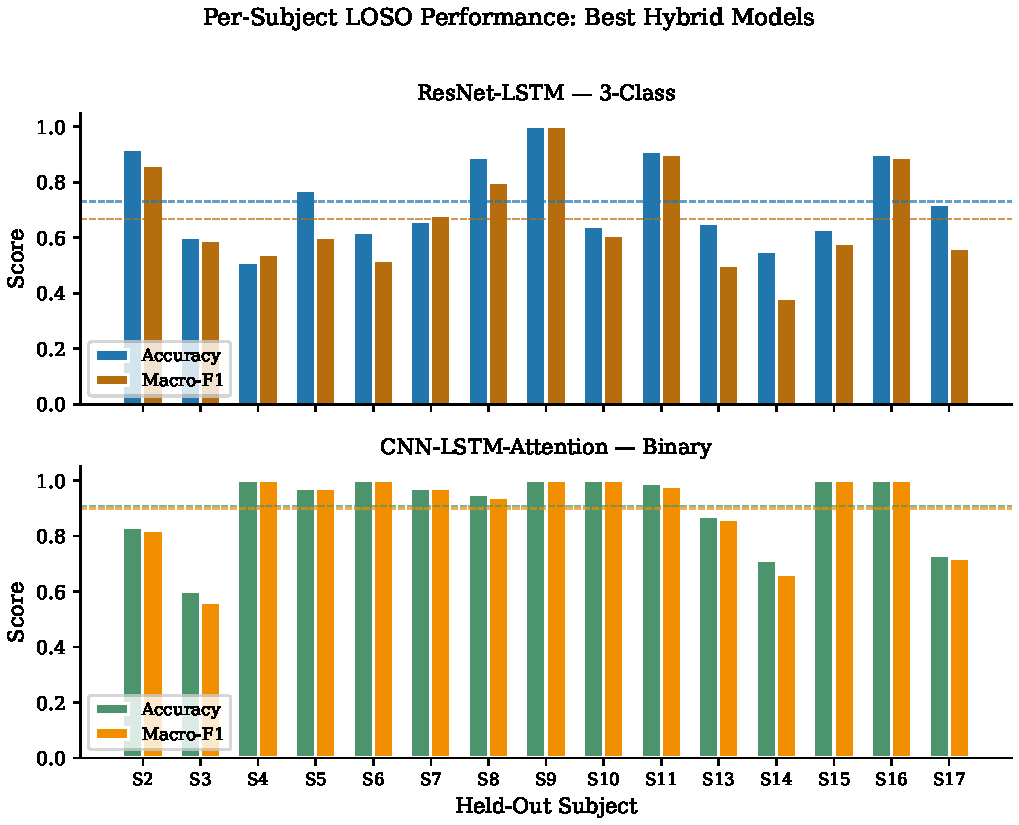
\includegraphics[width=0.85\linewidth]{hybrid_per_subject_loso.pdf}
\caption{Per-subject LOSO performance for the best hybrid models. \textbf{Top}: ResNet-LSTM (3-class)---S9 achieves perfect accuracy while S14 remains the hardest subject (F1 = 0.38). \textbf{Bottom}: CNN-LSTM-Attention (binary)---most subjects exceed 0.90 F1, but S3 (0.56) and S17 (0.72) remain outliers, mirroring the tabular results.}
\label{fig:hybrid-persub}
\end{figure}


\subsection{Cross-Pipeline Summary}

\begin{figure}[H]
\centering
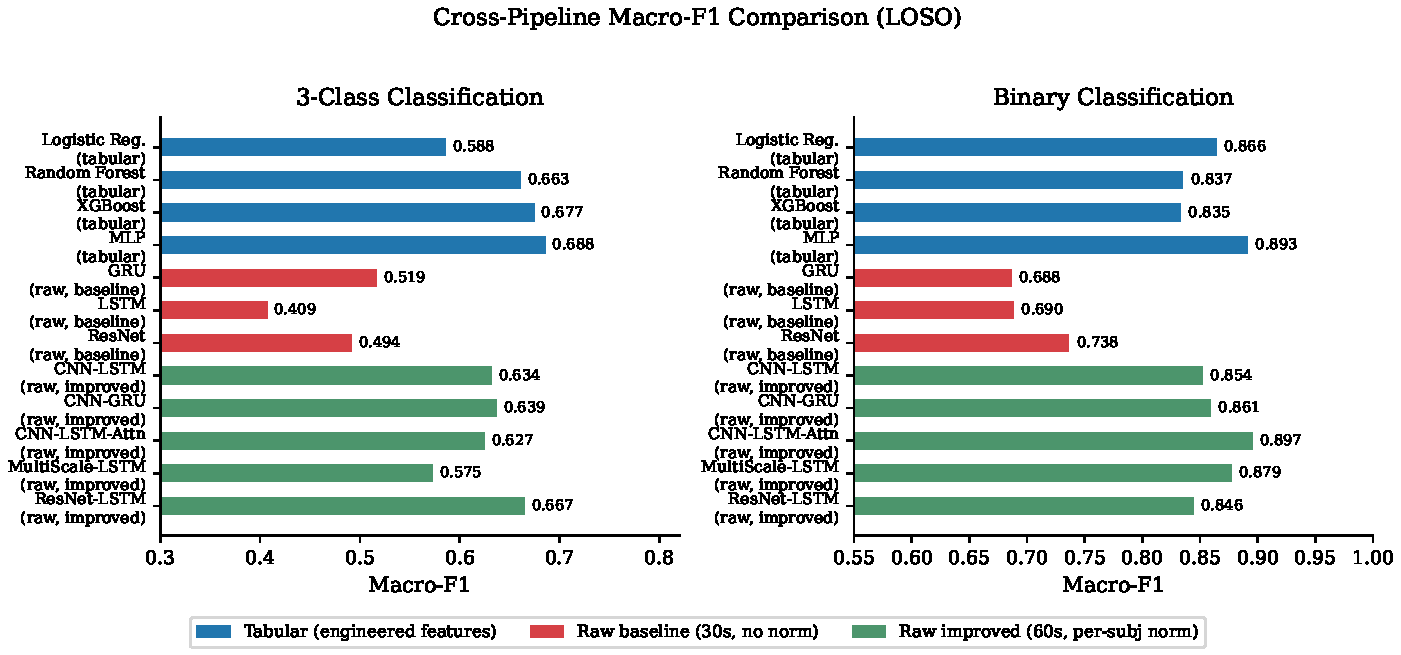
\includegraphics[width=0.95\linewidth]{grand_summary_comparison.pdf}
\caption{Macro-F1 across all 12 models grouped by pipeline. Tabular models on engineered features (blue) establish strong baselines; raw-signal baseline models (red) under-perform substantially; improved hybrid architectures (green) close the gap, with CNN-LSTM-Attention reaching 0.897 binary F1 (within 3\% of the tabular MLP) and ResNet-LSTM reaching 0.667 3-class F1 (within 1\% of XGBoost).}
\label{fig:grand-summary}
\end{figure}


% ======================================================================
\section{Discussion and Future Work}
\label{sec:discussion}
% ======================================================================

\subsection{Key Findings}

\begin{enumerate}
    \item \textbf{Engineered features remain competitive.}
    On the tabular pipeline, the MLP achieves 0.921 binary Macro-F1 and XGBoost achieves 0.677 3-class Macro-F1.
    These results demonstrate that carefully crafted summary statistics from physiological signals, combined with proper LOSO evaluation and class weighting, yield strong performance without requiring deep learning.

    \item \textbf{Naive end-to-end learning on raw wrist signals under-performs.}
    Standalone GRU, LSTM, and ResNet models achieve only 0.50--0.79 accuracy, significantly below tabular models.
    The low wrist sampling rate (4\,Hz for EDA/TEMP, 64\,Hz for BVP downsampled to 4\,Hz) limits the information density available to sequence models compared to hand-crafted features that compress domain knowledge.

    \item \textbf{Hybrid architectures and improved preprocessing close the gap.}
    The CNN-LSTM-Attention model achieves binary Macro-F1 of 0.897 on raw signals---within 3\% of the tabular MLP (0.921)---while the ResNet-LSTM achieves 3-class Macro-F1 of 0.667, nearly matching XGBoost (0.677).
    Per-subject normalisation, overlapping windows, and the combination of convolutional feature extraction with recurrent temporal modelling are the key enablers.

    \item \textbf{Amusement remains the hardest class.}
    Across all models and data representations, Amusement has the lowest F1 ($\leq$0.55 on tabular, $\leq$0.41 on raw signals), consistent with its small sample size (195/1178 = 16.6\%) and physiological overlap with Baseline.

    \item \textbf{High inter-subject variance persists.}
    All models exhibit standard deviations of $\pm$0.12--0.24 across LOSO folds.
    Certain subjects (S14, S17) remain difficult regardless of architecture, while others (S9, S10) are consistently well-classified, reflecting genuine inter-subject physiological differences.
\end{enumerate}

\subsection{Limitations}

\begin{itemize}
    \item \textbf{Small sample size}: 15 subjects limits the stability of LOSO estimates and prevents reliable hyperparameter tuning (no validation set distinct from test).
    \item \textbf{Wrist-only signals}: Chest sensors (ECG, EMG, respiration) provide richer physiological information but are excluded to focus on consumer-wearable feasibility.
    \item \textbf{Lab setting}: The controlled protocol may not generalise to free-living stress detection, where confounds (exercise, caffeine, sleep deprivation) are harder to control.
    \item \textbf{No hyperparameter search}: All model configurations use fixed hyperparameters without systematic tuning, which may leave performance gains on the table.
\end{itemize}

\subsection{Future Work}

\begin{itemize}    \item \textbf{Transformer-based architectures}: Multi-head self-attention models (e.g., temporal transformers) could better capture long-range dependencies without the sequential bottleneck of LSTMs.
    \item \textbf{Multi-task learning}: Jointly predicting stress level and arousal/valence could regularise representations and improve minority-class detection.
    \item \textbf{Domain adaptation}: Transfer learning from a pre-trained model on a larger physiological dataset (e.g., MIMIC or PhysioNet) could improve generalisation with limited WESAD subjects.
    \item \textbf{Free-living evaluation}: Validating models on uncontrolled, in-the-wild stress datasets would test real-world applicability.
    \item \textbf{Interpretability}: Attention weight visualisation and SHAP-based feature attribution could provide clinical insight into which temporal patterns drive predictions.
\end{itemize}


% ======================================================================
\begin{thebibliography}{9}
% ======================================================================

\bibitem{schmidt2018wesad}
P.~Schmidt, A.~Reiss, R.~D\"urichen, C.~Marberger, and K.~Van Laerhoven,
``Introducing WESAD, a multimodal dataset for wearable stress and affect detection,''
in \textit{Proc.\ 20th ACM Int.\ Conf.\ Multimodal Interaction (ICMI)}, 2018, pp.~400--408.

\bibitem{can2019stress}
Y.~S.~Can, N.~Chalabianloo, D.~Ekiz, and C.~Ersoy,
``Continuous stress detection using wearable sensors in real life: Algorithmic programming contest case study,''
\textit{Sensors}, vol.~19, no.~8, p.~1849, 2019.

\bibitem{siirtola2019continuous}
P.~Siirtola,
``Continuous stress detection using the sensors of commercial smartwatch,''
in \textit{Proc.\ ACM Int.\ Joint Conf.\ Pervasive and Ubiquitous Computing (UbiComp)}, 2019, pp.~1198--1201.

\bibitem{bobade2020stress}
P.~Bobade and M.~Vani,
``Stress detection with machine learning and deep learning using multimodal physiological data,''
in \textit{Proc.\ 2nd Int.\ Conf.\ Inventive Research in Computing Applications (ICIRCA)}, 2020, pp.~51--57.

\bibitem{sano2023cnnlstm}
M.~Sano, S.~Taylor, and R.~Picard,
``Deep learning based stress assessment using PPG signals,''
in \textit{Proc.\ IEEE Int.\ Conf.\ New Circuits and Systems (NEWCAS)}, 2023.

\bibitem{lin2023selfattention}
Y.~Lin, S.~Wang, and H.~Zhang,
``Deep CNN-LSTM with self-attention model for human activity recognition using wearable sensor,''
\textit{IEEE J.\ Biomed.\ Health Inform.}, vol.~26, no.~7, pp.~3127--3140, 2022.

\bibitem{fawaz2019resnet}
H.~I.~Fawaz, G.~Forestier, J.~Weber, L.~Idoumghar, and P.-A.~Muller,
``Deep learning for time series classification: A review,''
\textit{Data Min.\ Knowl.\ Discov.}, vol.~33, no.~4, pp.~917--963, 2019.

\bibitem{gjoreski2017monitoring}
M.~Gjoreski, H.~Gjoreski, M.~Lu\v{s}trek, and M.~Gams,
``Continuous stress detection using a wrist device: In laboratory and real life,''
in \textit{Proc.\ ACM Int.\ Joint Conf.\ Pervasive and Ubiquitous Computing (UbiComp) Workshops}, 2017, pp.~1185--1193.

\bibitem{indikawati2020stress}
F.~I.~Indikawati and S.~Winiarti,
``Stress detection from multimodal wearable sensor data,''
\textit{IOP Conf.\ Series: Materials Science and Engineering}, vol.~771, p.~012028, 2020.

\end{thebibliography}

\end{document}
